%#% extstart input preamble.tex
%
% memman.tex  Memoir class user manual (Part II only)  last updated 2009/09/07
%             Author: Peter Wilson
%             Copyright 2001, 2002, 2003, 2004, 2008, 2009 Peter R. wilson
%
%   This work has the LPPL maintenance status "maintained".
%   Maintainer: Lars Madsen (daleif at math dot au dot dk)
%
%\listfiles
\documentclass[10pt,letterpaper,extrafontsizes]{memoir}
\listfiles
\usepackage{comment}


% For (non-printing) notes  \PWnote{date}{text}
\newcommand{\PWnote}[2]{} 
\PWnote{2009/04/29}{Added fonttable to the used packages}
\PWnote{2009/08/19}{Made Part I a separate doc (memdesign.tex).}

% same
\newcommand{\LMnote}[2]{} 


\usepackage{memsty}
\usepackage{float}
%%%%%%%%%%%%%%%%%%%%%%%%%%%%
\usepackage{titlepages}  % code of the example titlepages
\usepackage{memlays}     % extra layout diagrams
\usepackage{dpfloat}     % floats on facing pages
\usepackage{fonttable}[2009/04/01]   % font tables
%%%%\usepackage{xr-hyper} \externaldocument{memdesign} Doesn't work, 
%%%%                      Idea won't work in general for memman/memdesign
%%%%                      as at display time, who knows where everything
%%%%                      will be located on the individual's computer.
%%%%%%%%%%%%%%%%%%%%%%%%%%%%

%%%% Change section heading styles
%%%\memmansecheads

%%%% Use the built-in division styling
%\headstyles{memman}

\pagenumbering{arabic}

%%% ToC down to subsections
\settocdepth{subsubsection}
%%% Numbering down to subsections as well
\setsecnumdepth{subsubsection}

%%%%%%%%%%%%%%%%%%%%%%% glossary
\makeglossary
\changeglossactual{?}
\changeglossnum{\@currentlabel} 
\changeglossnum{\thepage}
\changeglossnumformat{|hyperpage} %|
\renewcommand*{\glossaryname}{Command summary}
\renewcommand{\glossitem}[4]{%
  \sbox\@tempboxa{#1 \space #2 #3 \makebox[2em]{#4}}%
\par\hangindent 2em
  \ifdim\wd\@tempboxa<0.8\linewidth
    #1 \space #2 #3 \dotfill \makebox[2em][r]{#4}\relax
  \else
    #1 \dotfill \makebox[2em][r]{#4}\\
    #2 #3
  \fi}
\renewcommand*{\glossarymark}{\markboth{\glossaryname}{\glossaryname}}

%%%% extra index for first lines
\makeindex[lines]


% this 'if' is used to determine whether we are compiling the memoir
% master in the subversion repository, or the public memman.tex
\newif\ifMASTER
\MASTERfalse
%\MASTERtrue

\ifMASTER

% add patch to fink, such that \AtEndFile still work
\makeatletter
\AtEndFile{fink.sty}{
  \typeout{patching fink} 
  \renewcommand{\InputIfFileExists}[2]{%
    \IfFileExists{##1}%
    {##2\@addtofilelist{##1}%
      \m@matbeginf{##1}%
      \fink@prepare{##1}%
      %\@@input \@filef@und
      \expandafter\fink@input%
      \expandafter\fink@restore\expandafter{\finkpath}%
     \m@matendf{##1}%
     \killm@matf{##1}}%
 }
}
\makeatother
% private package, not in circulation
% enables us to gather svn information on a single file basis
%\usepackage[filehooks]{svn-multi-private}
% use the current version
%\usepackage[filehooks]{svn-multi}


% \svnidlong
% {}
% {$LastChangedDate: 2015-03-05 18:49:59 +0100 (Thu, 05 Mar 2015) $}
% {$LastChangedRevision: 516 $}
% {$LastChangedBy: daleif $}



%\makeatletter
%\newcommand\addRevisionData{%
%  \begin{picture}(0,0)%
%    \put(0,-20){%
%      \tiny%
%      \expandafter\@ifmtarg\expandafter{\svnfiledate}{}{%
%        \textit{\textcolor{darkgray}{Chapter last updated \svnfileyear/\svnfilemonth/\svnfileday
%         \enspace (revision \svnfilerev)}}
%     }%
%    }%
%  \end{picture}%
%}
%\makeatother

% we add this to the first page of each chapter

\makepagestyle{chapter}
\makeoddfoot{chapter}{\addRevisionData}{\thepage}{}
\makeevenfoot{chapter}{\addRevisionData}{\thepage}{}

\else
% disable svn info collecting
\newcommand\svnidlong[4]{}
\fi



%% end preamble
%%%%%%%%%%%%%%%%%%%%%%%%%%%%%%%%%%%%%%%%%%%%%%%%%%%%%%%
%#% extend

%\usepackage[draft]{fixme}
%\fxsetup{
%  layout=marginnote
%}
 

\begin{document}


%\tightlists
\firmlists
\midsloppy
\raggedbottom
%\chapterstyle{demo3}

%%%%%%%%%%%%%%%%%%%%%%%%%%%%%%%%%%%%%%%%%%%%%%%%%%%%%%%

%
\ProvidesFile{memnoidxnum}[2009/04/30  some index entries for memman]
\newcommand*{\idxat}{\index{@?\texttt{@}|noidxnum}} \idxat
%%\index{@?\texttt{@}|noidxnum}
\index{argument|noidxnum}
%%\index{array|noidxnum}
\index{cardinal|noidxnum}
\index{centering|noidxnum}
%%\index{chapterstyle|noidxnum}
%%\index{counter|noidxnum}
\index{default|noidxnum}
\index{division|noidxnum}
\index{division!sectional|seealso{subhead}}
\index{double column|noidxnum}
\index{endnote!mark|seealso{reference mark}}
\index{environment|noidxnum}
\index{error message|noidxnum}
\index{figures|noidxnum}
%%\index{file|noidxnum}
\index{font characteristic|noidxnum}
\index{footnote!mark|seealso{reference mark}}
\index{footnotes|noidxnum}
\index{frame|noidxnum}
\index{framed|noidxnum}
\index{full stop|seealso{period}}
\index{hanging|noidxnum}
\index{headstyles|noidxnum}
%%\index{horizontal|noidxnum}
\index{Hurenkinder|see{widow}}
\index{interlinear space|see{leading}}
\index{keyword|noidxnum}
%%\index{label|noidxnum}
\index{LaTeX?\ltx|noidxnum}
%%\index{length|noidxnum}
\index{line|noidxnum}
\index{line too long|see{overfull lines}}
\index{lining|noidxnum}
%%\index{list|noidxnum}
\index{lowercase|noidxnum}
\index{MakeIndex?\Pmakeindex|noidxnum}
\index{margin!spine|seealso{inner}}
\index{margin!inner|seealso{spine}}
\index{margin!foredge?\foredge|seealso{outer}}
\index{margin!outer|seealso{\foredge}}
\index{margin!upper|seealso{top}}
\index{margin!top|seealso{upper}}
\index{math|noidxnum}
%%\index{memoir class|noidxnum}
\index{minipage|noidxnum}
\index{name|noidxnum}
\index{named|noidxnum}
\index{new|noidxnum}
%%\index{number|noidxnum}
\index{numeric|noidxnum}
\index{old-style|noidxnum}
\index{option|noidxnum}
\index{ordinal|noidxnum}
\index{outline|noidxnum}
\index{package|noidxnum}
\index{page break|noidxnum}
%%\index{pagestyle|noidxnum}
\index{paragraph break|noidxnum}
\index{period|seealso{full stop}}
\index{poem|noidxnum}
\index{program|noidxnum}
\index{ranging|noidxnum}
\index{reference|noidxnum}
\index{reference mark|seealso{endnote mark, footnote mark}}
\index{representation|noidxnum}
\index{rule|noidxnum}
\index{ruled|noidxnum}
%%\index{section|noidxnum}
\index{Schusterjungen|see{orphan}}
\index{section|seealso{subhead}}
\index{sectional division|seealso{subhead}}
\index{single column|noidxnum}
\index{size|noidxnum}
\index{space|noidxnum}
\index{space!double|see(double spacing)}
\index{space!between lines|see{leading}}
\index{stanza|noidxnum}
%%\index{subfloat|noidxnum}
\index{TeX?\tx|noidxnum}
\index{text|noidxnum}
\index{titling|noidxnum}
\index{trim|noidxnum}
%%\index{type size|noidxnum}
\index{vertical|noidxnum}
\index{warning|noidxnum}
\index{write|noidxnum}
%%\index{XeTeX?\xetx|noidxnum}

%%%%%%%% Deleted the font indexing (now done as typefaces) 2009/04/30

\begin{comment}
\index{table of contents|see{ToC}}
\index{list!of figures|see{LoF}}
\index{figure!list of|see{LoF}}
\index{list!of tables|see{LoT}}
\index{table!list of|see{LoT}}
\index{marginal note|see{marginalia}}
\index{footnote!in title|see{thanks}}
\index{illustration|seealso{float, figure}}
\index{figure|seealso{float}}
\index{table|seealso{float}}
\index{chapter!style|see{chapterstyle}}
\index{chapter!heading|see{heading}}
\index{page!style|see{pagestyle}}
\index{part!heading|see{heading}}
\end{comment}

\begin{comment}

%%%% deleted the \nocites
%
\index{anonymous division|see{division}}
\index{array|seealso{tabular}}
%
\index{Berne Convention|see{copyright}}
\index{blank page|see{page}}
\index{Buenes Aires Convention|see{copyright}}
\index{box!rule|seealso{rule}}
%
\index{chapter|seealso{division}}
\index{chapter!style|see{chapterstyle}}
\index{command|seealso{declaration, macro}}
\index{comptexttex?\texttt{comp.text.tex} newsgroup|see{\ctt}}
\index{Comprehensive TeX Archive Network?\cTeXan|see{\ctan}}
\index{contents list|see{ToC}}
\index{counter representation!Alph tt?\texttt{Alph}|see{\texttt{Alph}}}
\index{counter representation!alph tt?\texttt{alph}|see{\texttt{alph}}}
\index{counter representation!arabic tt?\texttt{arabic}|see{\texttt{arabic}}}
\index{counter representation!Roman tt?\texttt{Roman}|see{\texttt{Roman}}}
\index{counter representation!roman tt?\texttt{roman}|see{\texttt{roman}}}
\index{counter representation!fnsymbol tt?\texttt{fnsymbol}|see{\texttt{fnsymbol}}}
\index{cross reference|seealso{reference}}
%
\index{descriptive list|see{list}}
\index{display math|see{math}}
\index{display mode|see{display}}
\index{division|seealso{heading}}
%
\index{electronic book|see{ebook}}
\index{enumerated list|see{list}}
%
\index{figure!list of|see{LoF}}
\index{figure|seealso{float}}
\index{float!numbered captioning|see{caption}}
\index{float!unnumbered captioning|see{legend}}
\index{font characteristic!weight|see{series}}
%
\index{file|seealso{stream}}
\index{footnote!in title|see{thanks}}
\index{fragile command|seealso{protect}}
\index{free tabular|seealso{tabular}}
%
\index{header|seealso{running header}}
\index{heading|seealso{division}}
%
\index{illustration|seealso{float, figure}}
\index{inline math|see{math}}
\index{International Standard Book Number|see{ISBN}}
\index{itemized list|see{list}}
%
\index{label|seealso{reference}}
\index{left-to-right|see{LR}}
\index{list!new list of|see{list of, new}}
\index{list!of contents|see{ToC}}
\index{list!of figures|see{LoF}}
\index{list!of tables|see{LoT}}
\index{list of!contents|see{ToC}}
\index{list of!figures|see{LoF}}
\index{list of!tables|see{LoT}}
\index{LoF|seealso{ToC}}
\index{LoT|seealso{ToC}}
\index{log-like function|see{function}}
%
\index{macro|seealso{command}}
\index{margin note|seealso{marginalia}}
\index{marginalia|seealso{marginal note, side note, sidebar}}
%
\index{named division|see{division}}
%
\index{page!of floats|see{float, page}}
\index{page!start new|see{start new page}}
\index{page!style|see{pagestyle}}
\index{paragraph|seealso{division}}
\index{part|seealso{division}}
\index{picture object!Bezier curve|see{Bezier curve}}
\index{picture object!circle|see{circle}}
\index{picture object!line|see{line}}
\index{picture object!oval|see{box, rounded}}
\index{picture object!vector|see{vector}}
\index{poem|see{verse}}
\index{poetry|see{verse}}
\index{print run|see{impression}}
\index{protect|seealso{fragile command}}
%
\index{recto|seealso{odd page}}
\index{reference|seealso{label}}
\index{river|see{white space}}
\index{rivulet|see{white space}}
\index{running footer|see{footer}}
\index{running header|seealso{header}}
%
\index{section|seealso{division}}
\index{side note|seealso{marginalia}}
\index{sidebar|seealso{marginalia}}
\index{stanza|seealso{verse}}
\index{stanza!line number|see{line number}}
\index{subparagraph|seealso{division}}
\index{subsection|seealso{division}}
\index{subsubsection|seealso{division}}
%
\index{table of contents|see{ToC}}
\index{table!list of|see{LoT}}
\index{table|seealso{float}}
\index{tabular|seealso{array}}
\index{tabular!free|see{free tabular}}
\index{tabulation|see{tabular}}\
\index{TeX Users Group?\TeXUG|see{\tug}}
\index{textblock|see{typeblock}}
%
\index{Universal Copyright Convention|see{copyright}}
%
\index{verbatim!line number|see{line number}}
\index{verse|seealso{stanza}}
\index{verse!title|see{poem title}}
\index{verse!line number|see{line number}}
\index{verso|seealso{even page}}
\index{visual markup|see{visual design}}
%
\index{x coordinate|see{coordinate}}
%
\index{y coordinate|see{coordinate}}
%
%


\end{comment}

\endinput



\frontmatter
\pagestyle{empty}


% title page
\vspace*{\fill}
\begin{center}
\HUGE\textsf{ATSDB}\par
\end{center}

\begin{center}
\Huge\textsf{User Guide}\par
\end{center}
\begin{center}
\normalsize\textsf{Maintained by Helmut Puhr}\par
\medskip
\normalsize\textsf{Version 0.0.9 \textit{Befuddled Badger}}\par
\end{center}
\vspace*{\fill}
\begin{center}

\includegraphics[width=\droptitle]{../logo/atsdb.png}
\setlength{\droptitle}{0pt}%
\end{center}
\clearpage

\cleardoublepage

% ToC, etc
%%%\pagenumbering{roman}
\pagestyle{headings}
%%%%\pagestyle{Ruled}

\setupshorttoc
\tableofcontents
\clearpage
\setupparasubsecs
\setupmaintoc
\tableofcontents
\setlength{\unitlength}{1pt}
\clearpage
\listoffigures
\clearpage
\listoftables

%#% extend

\chapter{Introduction}

This document has its focus on interaction and working procedures required to make use of the existing
functionality. In this introduction, feature highlights are listed, followed by a brief summary of important aspects of  ATSDB. In the later section \nameref{sec:usage}, a functional, task-oriented overview is given. 
%At the end of the document, a glossary is given.

\section{Feature highlights}

The \textbf{A}ir \textbf{T}raffic \textbf{S}urveillance \textbf{D}ata\textbf{B}ase aims at providing a generalized framework for ATM surveillance data inspection. While its current functionality is somewhat limited, the following features exist:\\\\

\begin{itemize}  
\item Support of multiple database systems, e.g. SCDB
\item High performance processing, low memory footprint
\item Utilization of application during loading procedure
\item Views for data inspection
\item Simple custom filter generation
\item Supported Database Objects
\begin{itemize}  
\item Radar plots
\item System Tracks and Reference Trajectories
\item MLAT \& WAM target reports
\item ADS-B target reports
\end{itemize}
\item XML-based configuration files
\item Multiple coexisting configurations, usage chosen during runtime
\item Based on Open Source libraries
\item Runs on generic hardware
\end{itemize}

There also exists an integrated display solution, called the ATSDB display. Currently it is experimental, and still under heavy development. For this reasons, it is not released as source code, but can be downloaded as an AppImage as binary component only. Please note that the display functionality is described in the later chapter OSG View (in section \ref{sec:osg_view}). The following features currently exist:

\begin{itemize}  
\item High-performance display based on OpenSceneGraph
\item Customizable map/terrain display based on osgEarth
\item Customizable display of Database Objects
\item Selection and labeling
\item Relatively low memory footprint (e.g. 17 million target reports in 6 GB RAM)
\end{itemize}

\section{General Aspects}
ATSDB is a highly specialized surveillance data processing framework, with a strong focus on high-performance and  a  low  memory  footprint,  to  process  massive  quantities  of  data.   Surveillance  data  is fetched from a database (limited by a filter system), then processed and displayed using so-called Views (visualization of aspects of the result set).\\\\

As storage medium, a database is used.  Different database systems are supported, and a flexible read-out system allows for easy adaptation to different database schemas.  Data in such a database has to be generated in a previous, separate process.  One method would be to use EUROCONTROLS SASS-C  Verif V7/8 framework.\\

When such a previously generated database is opened for the first time, some post-processing is performed, to ease usage and to increase startup speed.  When data is loaded using a database query, a filter configuration may restrict the data leading to a result set.  Such a result set can be analyzed using Views, e.g. the Listbox view.\\

Each View defines which parts of the database are required to fulfill its purpose, and only such parts are loaded.  During a loading process from the database, subsets of the query result are immediately added to the current result set and all views are updated.

\chapter{Key Concepts}
\label{cha:key_concepts}

In this section, a few key concepts are introduced to give a somewhat deeper understanding of ATSDB and to allow the reader to understand some main design choices made by the author. This should also give indications about the strengths and draw-backs of the chosen approach.

\section*{Database Systems}
A database allows for storage, retrieval and filtering of the data of interest. While SQL has some definitive drawbacks, it was chosen since support of the SASS-C database SCDB was wanted.\\
Currently  two  database  systems  are  supported:  MySQL  and  SQLite3.   MySQL  relies  on  an  independent background process, which holds several databases and can also be accessed over a network connection.\\
SQLite3 encapsulates one database in a single file container, which is read from a storage medium (e.g. hard drive).

\section*{Configuration}
At startup, several configuration files are loaded, and at shutdown the current configuration state of ATSDB is saved.  But configuration is not just a matter of components having the same parameters, but also what components exist. To give an example: Each existing View is saved, and when the program is started again, the previously active Views are created.  The same holds for the filters, or the database interface/schema. \\
This way, a user can have a specific program configuration for a specific usage situation, which can be instantly reused for a different dataset, using have a completely configurable database schema or filter configuration. \\
This allows for a high degree of flexibility, but somewhat complicates software development.

\section*{Flexible Database Interface}
Using such a configuration, a flexible database interface method was implemented to allow general displaying of data in different database systems and schemas.  How this was done would require a detailed discussion, which will be skipped for the moment.\\
To summarize, several database schemas can be stored in configuration files, each of which is a structured collection of database tables and their logical dependencies. Such information is used in one set of Database Objects (DBOs). In each database system, any database schema can be used.

\section*{Database Objects}
A Database Object (DBO) is defined by a name and has a collection of variables. For example, radar plots and system tracks are database objects, and each has variables holding time, position, Mode 3/A codes and Mode C heights and so on. From a database, if such a DBO is present, it can be loaded and displayed.\\

To allow displaying data from different DBOs in the same system, so-called meta-variables were  introduced, which hold variables that are present in some or all DBOs (with a possibly different name or unit).  For example, there meta-variable 'tod', which is a collection of sub-variables for each existing DBO and the respective ``Time of Day'' variable.

\section*{Data Loading}
In ATSDB, a unified data loading process was chosen, meaning that only exactly one common dataset is loaded, which can be inspected using Views. When started, data is incrementally read from the database, stored in the resulting dataset, and distributed to the active Views. Each time such a loading process is triggered, all Views clear their dataset and gradually update. \\
This makes working with the data somewhat easier to understand, since only one dataset exists, while on the other hand it does not allow several independent datasets (e.g. with different filters) to be loaded.

\section*{Generating a Database}
\label{sec:generation}

A database has to be generated before it can be opened with ATSDB.  This section describes how such
a process can be performed, however it is by no means a complete guide.

\section*{SASS-C Verif}
A complete treatment of how to generate a database using the highly sophisticated SASS-C Verif frame work  is  out  of  the  scope  of  this  document.   However,  a  short  summary  of  the  necessary  steps  will  be presented here.\\

\begin{itemize}  
\item Import a previous evaluation job
\item Set data recording path, e.g. 'somelocation/\%iffile.if'
\item Run IRIS command
\item Run OTR command
\item Run CMP command with all but RA
\item Run CMP command with just RA
\end{itemize}

After  these  steps,  a  database  was  generated  and  filled  with  data.   The  name  of  the  database  (which
will  be  needed  during  the  opening  process)  is  equivalent  to  the  job  name,  e.g.   'job\_v7\_mainsacso\_0005', 'HelloWorld' etc. \\

Please \textbf{note} that the SASS-C MySQL database name is not case sensitive ('job\_v7\_mainsacso\_0005' is the same as 'JOB\_V7\_MAINSACSO\_0005').

\chapter{Installation}
\label{sec:installation}

ATSDB can either be built from source (which exludes the OSG View, but allows development of additional features), or downloaded as an AppImage (binary distributable which includes the OSG View). The recommended option for non-developers is the AppImage.

\section{Using the AppImage}

To summarize, an AppImage is a form of binary distribution in one complete package, which does not require installation of any libraries or alteration of the operating system. Please refer to \url{https://appimage.org/} to get additional information.

To obtain the ATSDB AppImage, download the most current distribution from TODO. To execute, make it executable using the following command:
\begin{verbatim}
chmod +x ATSDB-x86_64_release.AppImage
\end{verbatim}

Generally speaking, that is it. The application can be run using the following command:
\begin{verbatim}
./ATSDB-x86_64_release.AppImage -f
\end{verbatim}

The following notes that should be considered:

\begin{itemize}  
\item The AppImage should run under any Linux distribution of similiar date to Ubuntu 14.04 or later, but no guarantees can be made.
\item The AppImage performance is somewhat lessened in comparison to the a later Ubuntu version, which in all probability is just that the graphics system is that outdated. This will be investigated further.
\item OSG View rendering is performed according to the local graphics card and driver, and might be limited by their capabilities.
\end{itemize}

\section{Building from Source Code}
Currently, ATSDB can be installed as source code and compiled by the user. Any recent Linux installation should work without issues. Regarding software version, no particularly new features were used, so older versions than the verified ones should also work. \\

The following software has to be installed on the workstation:

\begin{table}[H]
  \center
  \begin{tabular}{ | l | l | l |}
    \hline
    \textbf{Package} & \textbf{Description} & \textbf{Verified version} \\ \hline
    g++ & C++11 capable C++ compiler & 7.2.0 \\ \hline
    cmake & CMake build tool & 3.9.1 \\ \hline
    qt5-default & Qt5 development package & 5.9.1 \\ \hline
    libboost-dev & Boost development libraries & 1.62.0.1 \\ \hline
    mysql++-dev & MySQL library bindings & 3.2.2 \\ \hline
    libmysqlclient-dev & MySQL development library & 1.0.2 \\ \hline
    libsqlite3-dev & Sqlite3 development files & 3.2.2 \\ \hline
    libgdal-dev & Geospatial data abstraction library & 2.2.1 \\ \hline
    tinyxml2-dev & XML parsing library & 5.0.1 \\ \hline
    log4cpp5-dev & Logging libary & 1.1.1 \\ \hline
    doxygen & Documentation generation & 1.8.13 \\ 
    \hline
  \end{tabular}
  \caption{Required software/libraries}
\end{table}

To install to source code, either download the latest released version from \\ \url{https://github.com/hpuhr/ATSDB/releases} \\
or use the following command (git required) to clone the current repository:

\begin{verbatim}
git clone https://github.com/hpuhr/ATSDB.git
\end{verbatim}

Enter the ATSDB source folder, and execute cmake to create a Makefile:

\begin{verbatim}
cmake .
\end{verbatim}

The output should look like this:
\begin{verbatim}
sk@golem:~/test/ATSDB$ cmake .
  Path: /home/sk/test/ATSDB
-- The C compiler identification is GNU 7.2.0
-- The CXX compiler identification is GNU 7.2.0
-- Check for working C compiler: /usr/bin/cc
-- Check for working C compiler: /usr/bin/cc -- works
-- Detecting C compiler ABI info
-- Detecting C compiler ABI info - done
-- Detecting C compile features
-- Detecting C compile features - done
-- Check for working CXX compiler: /usr/bin/c++
-- Check for working CXX compiler: /usr/bin/c++ -- works
-- Detecting CXX compiler ABI info
-- Detecting CXX compiler ABI info - done
-- Detecting CXX compile features
-- Detecting CXX compile features - done
  System: Linux-4.13.0-16-generic
  Install Path: /home/sk/test/ATSDB/dist
  Platform: Linux
-- Looking for pthread.h
-- Looking for pthread.h - found
-- Looking for pthread_create
-- Looking for pthread_create - not found
-- Looking for pthread_create in pthreads
-- Looking for pthread_create in pthreads - not found
-- Looking for pthread_create in pthread
-- Looking for pthread_create in pthread - found
-- Found Threads: TRUE  
-- Boost version: 1.62.0
-- Found the following Boost libraries:
--   regex
--   system
--   thread
--   chrono
--   date_time
--   atomic
  Boost_INCLUDE_DIR: /usr/include
  Boost_LIBRARY_DIR: 
  CMAKE_MODULE_PATH: /home/sk/test/ATSDB/cmake_modules
-- Found MySQL: /usr/lib/libmysqlpp.so
  MySQLpp_INCLUDE_DIR: /usr/include/mysql++
  MySQLpp_LIBRARY: /usr/lib/libmysqlpp.so
-- Found MySQL: /usr/lib/x86_64-linux-gnu/libmysqlclient.so
  MYSQL_INCLUDE_DIR: /usr/include/mysql
-- Found Sqlite3 header file in /usr/include
-- Found Sqlite3 libraries: /usr/lib/x86_64-linux-gnu/libsqlite3.so
  SQLite3_INCLUDE_DIR: /usr/include
  SQLite3_LIBRARY_DIR: /usr/lib/x86_64-linux-gnu/libsqlite3.so
-- Found Log4CPP
  LOG4CPP_INCLUDE_DIR: /usr/include
  LOG4CPP_LIBRARY: /usr/lib/x86_64-linux-gnu/liblog4cpp.so
-- Found GDAL: /usr/lib/libgdal.so  
  GDAL_INCLUDE_DIRS: /usr/include/gdal
  GDAL_LIBRARIES: /usr/lib/libgdal.so
  TINYXML2_INCLUDE_DIR: /usr/include
  TINYXML2_LIBRARY: /usr/lib/x86_64-linux-gnu/libtinyxml2.so
-- Found Doxygen: /usr/bin/doxygen (found version "1.8.13") found components:  doxygen 
CPACK_SOURCE_IGNORE_FILES = /CMakeFiles/;/_CPack_Packages/;/dist/;/.git/;
-- Configuring done
-- Generating done
-- Build files have been written to: /home/sk/test/ATSDB
\end{verbatim}

Then, compile the source by executing:

\begin{verbatim}
make
\end{verbatim}

The output should look like this:

\begin{verbatim}
Scanning dependencies of target atsdb_autogen
[  1%] Automatic MOC for target atsdb
Generating MOC predefs moc_predefs.h
Generating MOC source 2MJGWJB4P3/moc_mainwindow.cpp
...
Generating MOC source 3JYSCEOBDA/moc_viewmanagerwidget.cpp
Generating MOC compilation mocs_compilation.cpp
[  1%] Built target atsdb_autogen
Scanning dependencies of target atsdb
[  2%] Building CXX object CMakeFiles/atsdb.dir/src/atsdb.cpp.o
[  2%] Building CXX object CMakeFiles/atsdb.dir/src/buffer/arraylist.cpp.o
...
[ 93%] Linking CXX shared library dist/lib/libatsdb.so
[ 93%] Built target atsdb
Scanning dependencies of target atsdb_client_autogen
[ 94%] Automatic MOC for target atsdb_client
Generating MOC predefs moc_predefs.h
Generating MOC source 2MJGWJB4P3/moc_mainwindow.cpp
...
Generating MOC source 3JYSCEOBDA/moc_viewmanagerwidget.cpp
Generating MOC compilation mocs_compilation.cpp
[ 94%] Built target atsdb_client_autogen
Scanning dependencies of target atsdb_client
...
[100%] Linking CXX executable atsdb_client
[100%] Built target atsdb_client
\end{verbatim}

To install the ATSDB client, execute the following command in the build folder:

\begin{verbatim}
sudo make install
\end{verbatim}

This will install binary and a data folder to your system directories, commonly in '/usr/local/bin/', '/usr/local/lib/' and '/usr/local/atsdb/' (or similiar, depending on you Linux distribution.

To start the ATSDB client execute:

\begin{verbatim}
atsdb_client
\end{verbatim}

\chapter{Usage}
\label{sec:usage}

\section{Opening a database}
\label{sec:startup}

While ATSDB is more a database framework, it comes with a dedicated client. When the ATSDB client is started a dialog  for opening a database is shown. 

\begin{figure}[H]
  \hspace*{-2cm}
    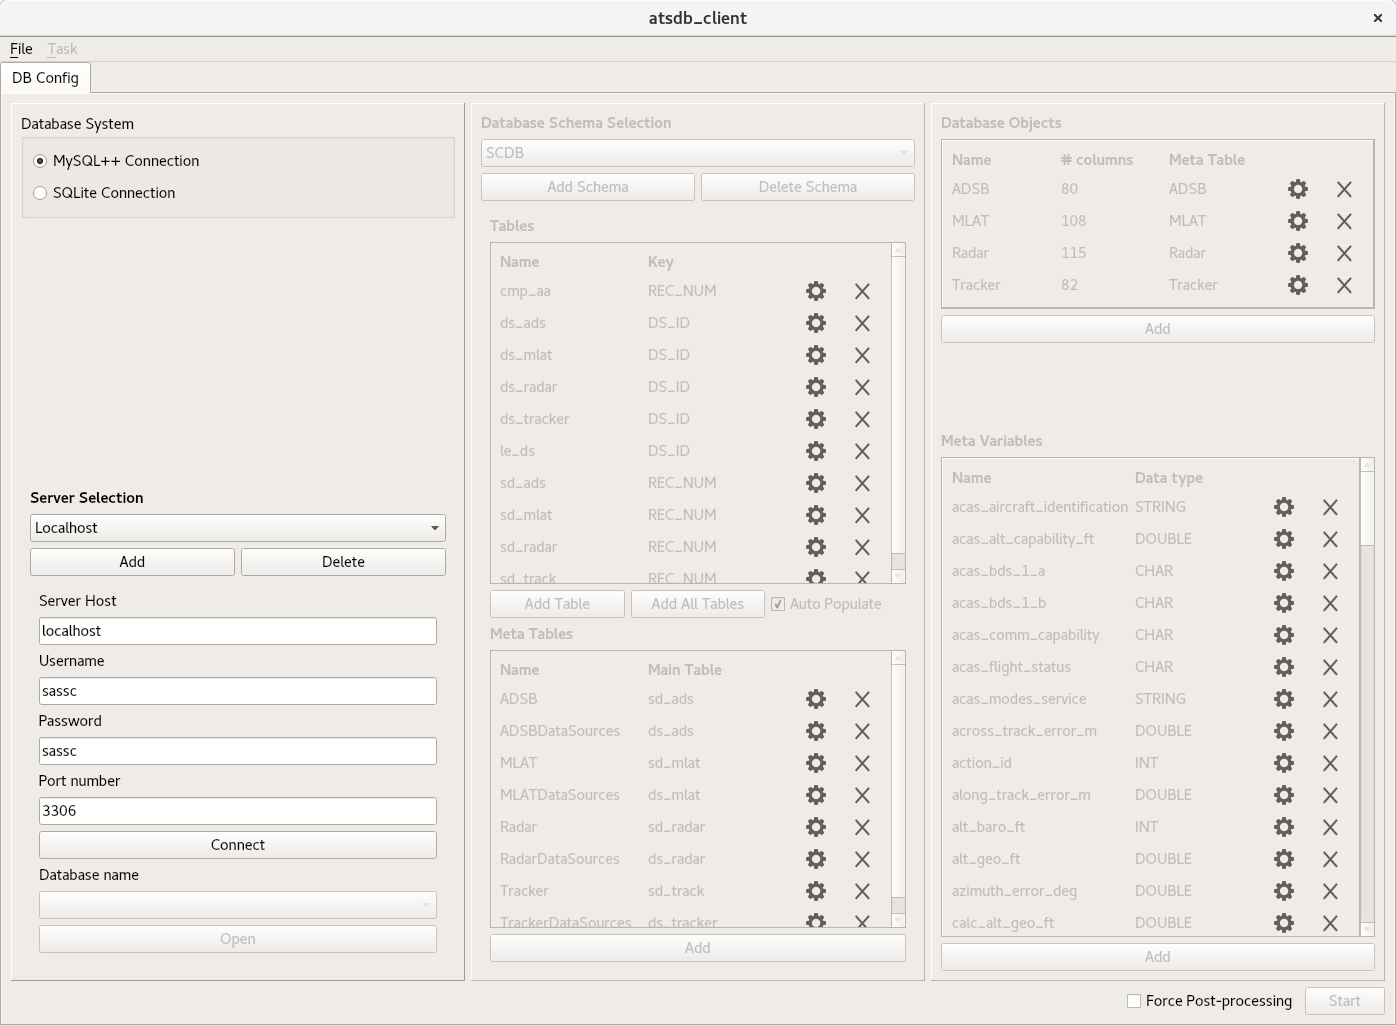
\includegraphics[width=18cm]{../screenshots/db_config_connect.png}
  \caption{Connecting to a database}
  \label{fig:db_connect}
\end{figure}

On the left-hand side, a database system can be selected.  Choices are either MySQL database or a file container with a SQLite3 database. \\
On the lower left (depending on the database system) either a MySQL server connection can be configured or a list of SQLite3 files is shown.\\

On the right-hand side a database schema can be selected and edited (editing is only recommended for experienced users).

\subsection{Database Selection}
\subsubsection{MySQL database}

\begin{figure}[H]
  \center
    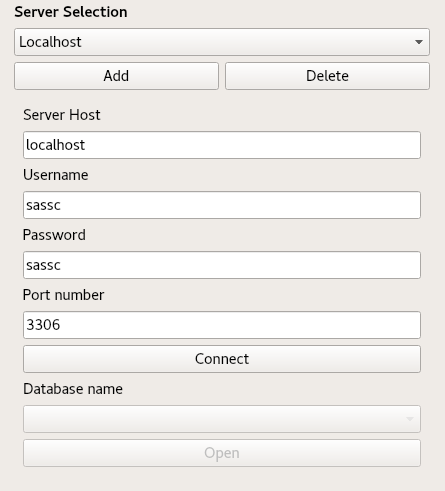
\includegraphics[width=8cm]{../screenshots/mysql_server_selection.png}
  \caption{Connecting to a MySQL server}
  \label{fig:mysql_connect}
\end{figure}

Several MySQL servers can be defined, each one has a specific set of parameters. To add a new server, press the 'Add' button and enter a unique server name. To select the currently used server, use the dropdown menu. To delete the currently used server, press the 'Delete' button.

For connecting to a MySQL database, several parameters have to be entered:

\begin{table}[H]
  \center
  \begin{tabular}{ | l | l | l |}
    \hline
    \textbf{Parameter} & \textbf{Description} & \textbf{Example Values} \\ \hline
    Server Host & Network identifier of server & 'localhost', '10.0.0.123' \\ \hline
    Username & MySQL user name & 'sassc', 'root' \\ \hline
    Password & MySQL user password & 'sassc', '' \\ \hline
    Port Number & MySQL server port & '3306', '' \\
    \hline
  \end{tabular}
  \caption{MySQL server parameters}
\end{table}

To connect to a defined MySQL server, press the 'Connect' button.\\

Please note that it is not recommended to use SASS-C databases on which actual performance evaluations are to be performed. Using ATSDB, database operations can be performed which might impede results later obtained by using SASS-C. For this reason, it is recommended to either clone an evaluation or use one on which no later SASS-C evaluations are performed.

If a remote server is used, e.g. a SASS-C workstation, remote access might be prohibited, which will result in an access permissions error during connecting. To resolve this, (generally) remote access can be enabled in the servers MySQL configuration. As a superuser, edit the file 'my.cnf', which is commonly found under '/etc/mysql/my.cnf'. 

Find the line that states:
\begin{verbatim}
bind-address = 127.0.0.1
\end{verbatim}

Change the line to:

\begin{verbatim}
#bind-address = 127.0.0.1
\end{verbatim}

Then, restart the MySQL server using one the following commands:

\begin{verbatim}
/etc/init.d/mysqld restart

#OR, depending on your distribution
service mysql restart
\end{verbatim}

Then, to allow access to the databases, log into a MySQL client on the server as root and execute the following commands:

\begin{verbatim}
# log in as root, must be done as superuser
mysql -u root

# grant access rights for your MySQL user, 
# e.g. 'sass', from the your local IP address, 
# e.g. '192.168.0.104', using your password, e.g. 'sassc'
GRANT ALL ON *.* to' 'sassc'@'192.168.0.104' IDENTIFIED BY 'sassc';

# set access rights
FLUSH PRIVILEGES;

# exit the MySQL client
exit
\end{verbatim}

After executing these steps once, remote access to this MySQL server from the specified IP address is enabled.

If  a  wrong  database  name  or  IP  address  is  used,  error  messages  can  be  e.g.  \\

\begin{verbatim}
MySQLConnection: executeSQL: error when executing
\end{verbatim}
 or 
\begin{verbatim}
MySQLConnection:  init:  DB connection failed
\end{verbatim} 

If such an error occurs, correcting the server host name and or user/password should solve the problem.

After successful connection, all existing databases in the server are shown in the 'Database name' drop-down menu. The last used one is selected automatically.

\begin{figure}[H]
  \center
    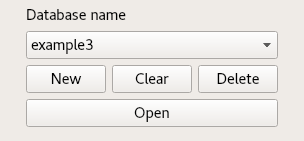
\includegraphics[width=8cm]{../screenshots/mysql_database_selection.png}
  \caption{Selecting a MySQL database.}
  \label{fig:mysql_db_select}
\end{figure}


To open a database click the 'Open' button (lower left corner).

\subsubsection{SQlite3 File container}
For opening a file container, clicking the 'Select' button opens a file selection dialog, in which any SQLite3 file can be selected as data source.

\begin{figure}[H]
  \center
    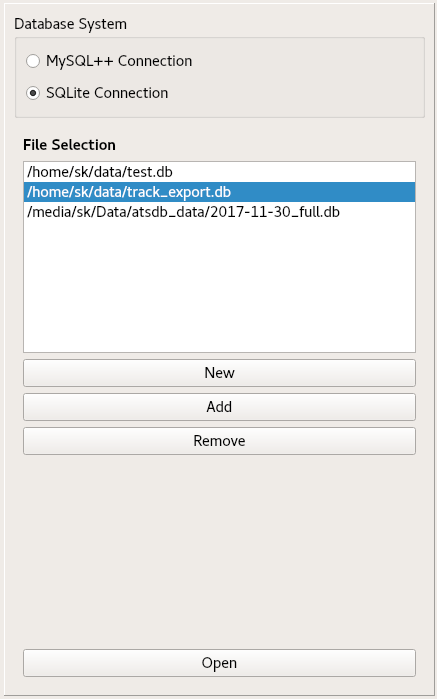
\includegraphics[width=8cm]{../screenshots/sqlite3_open.png}
  \caption{Opening a SQLite3 file container}
  \label{fig:sqlite3_open}
\end{figure}

\subsection{Database Schema Selection}
For a common user, selection of a pre-configured database schema is recommened. To select a different database schema, please use the 'Schema selection' drop-down menu.\\

\begin{figure}[H]
  \center
    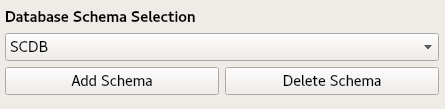
\includegraphics[width=8cm]{../screenshots/database_schema_selection.png}
  \caption{Selecting a database schema}
  \label{fig:db_schema_select}
\end{figure}

For experienced users, on the right-hand side a database schema can be selected and edited, which is currently not recommended (since it is not user friendly and might crash if used in the ``wrong'' manner).

\begin{figure}[H]
  \hspace*{-1cm}
    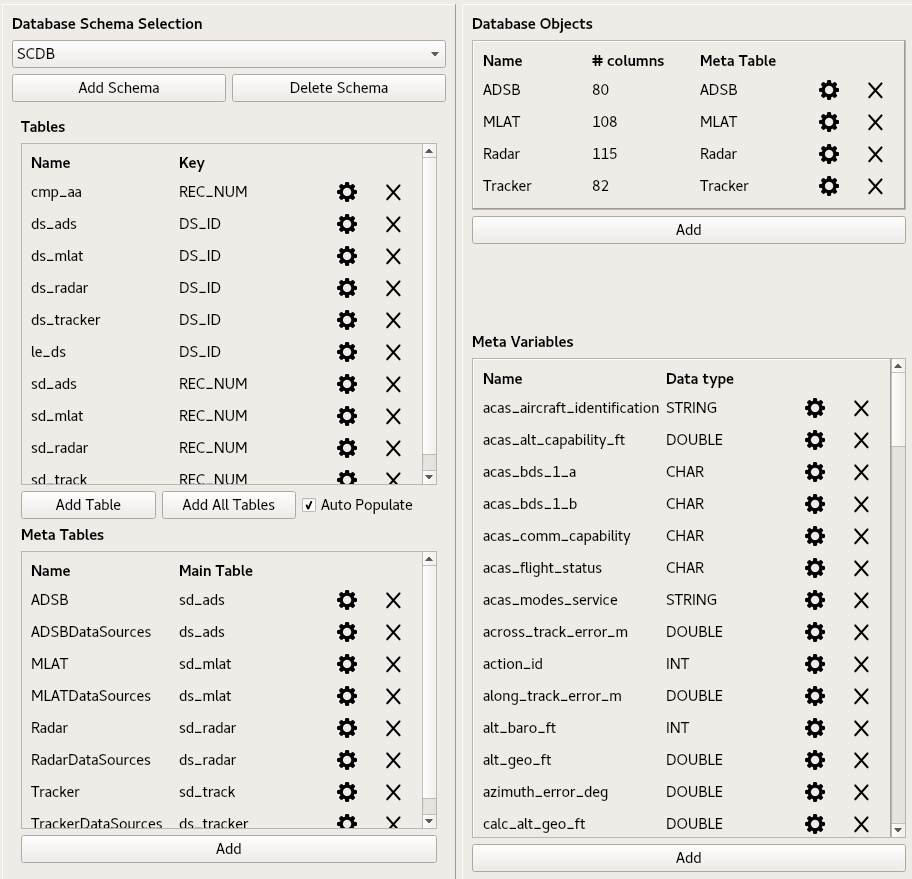
\includegraphics[width=16cm]{../screenshots/database_schema_configuration.png}
  \caption{Configuring a database schema}
  \label{fig:db_schema_configuration}
\end{figure}

\subsection{Starting}

After the previous steps have been completed, the 'Start' button can be pressed to continue. \\

When a database is opened the first time, a post-processing has to be performed.

\subsubsection{Postprocessing}
When a database is generated by a previous process,  some information that eases usage of the software does not exist. This information is generated once during a post-processing step, which is automatically performed. If wanted, it can always performed using the 'Force post-processing' checkbox.

Please \textbf{note} that during post-processing the application will not react to user input. \\


\begin{figure}[H]
  \hspace*{-2cm}
    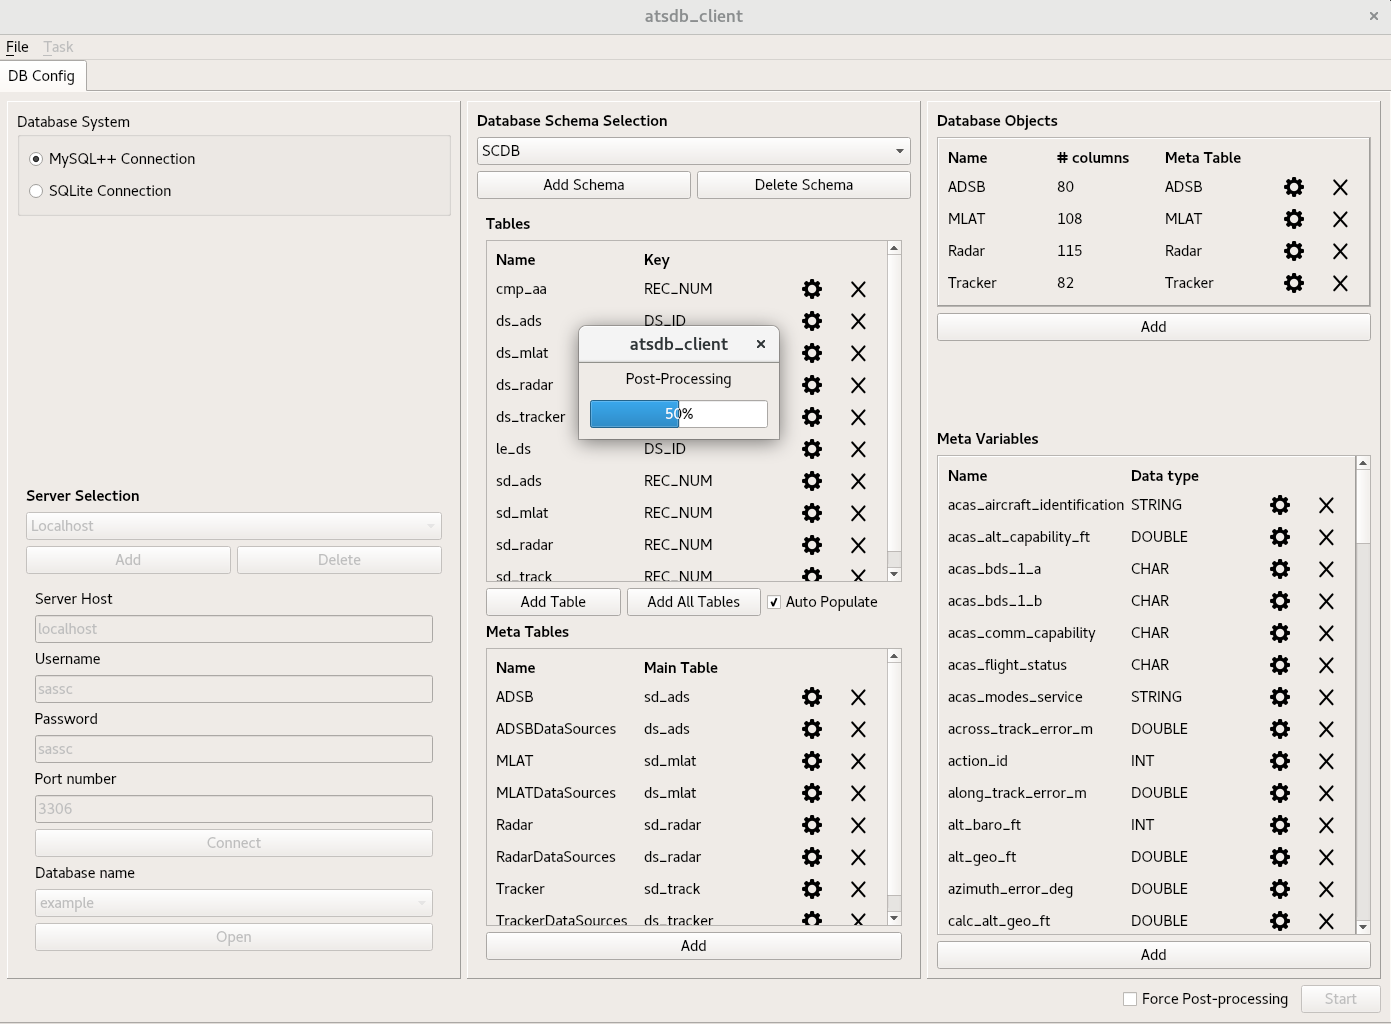
\includegraphics[width=18cm]{../screenshots/db_postprocessing.png}
  \caption{Post-processing a database}
  \label{fig:db_postprocessing}
\end{figure}

The following information is generated and stored in the database:

\begin{itemize}  
\item List of all active data sources for all DBOs
\item List with all minima/maxima for all variables of all DBOs
\end{itemize}

Please \textbf{note} that this step has to be performed only once for each database, and may take up to a few minutes for large datasets. \\

Please also \textbf{note} that during this step, no DBO data itself is changed, but only additional information is generated and stored in separate database tables.

\section{Management}
\label{sec:management}

After pressing the 'Start' button, a management window is shown.

\begin{figure}[H]
  \hspace*{-2cm}
    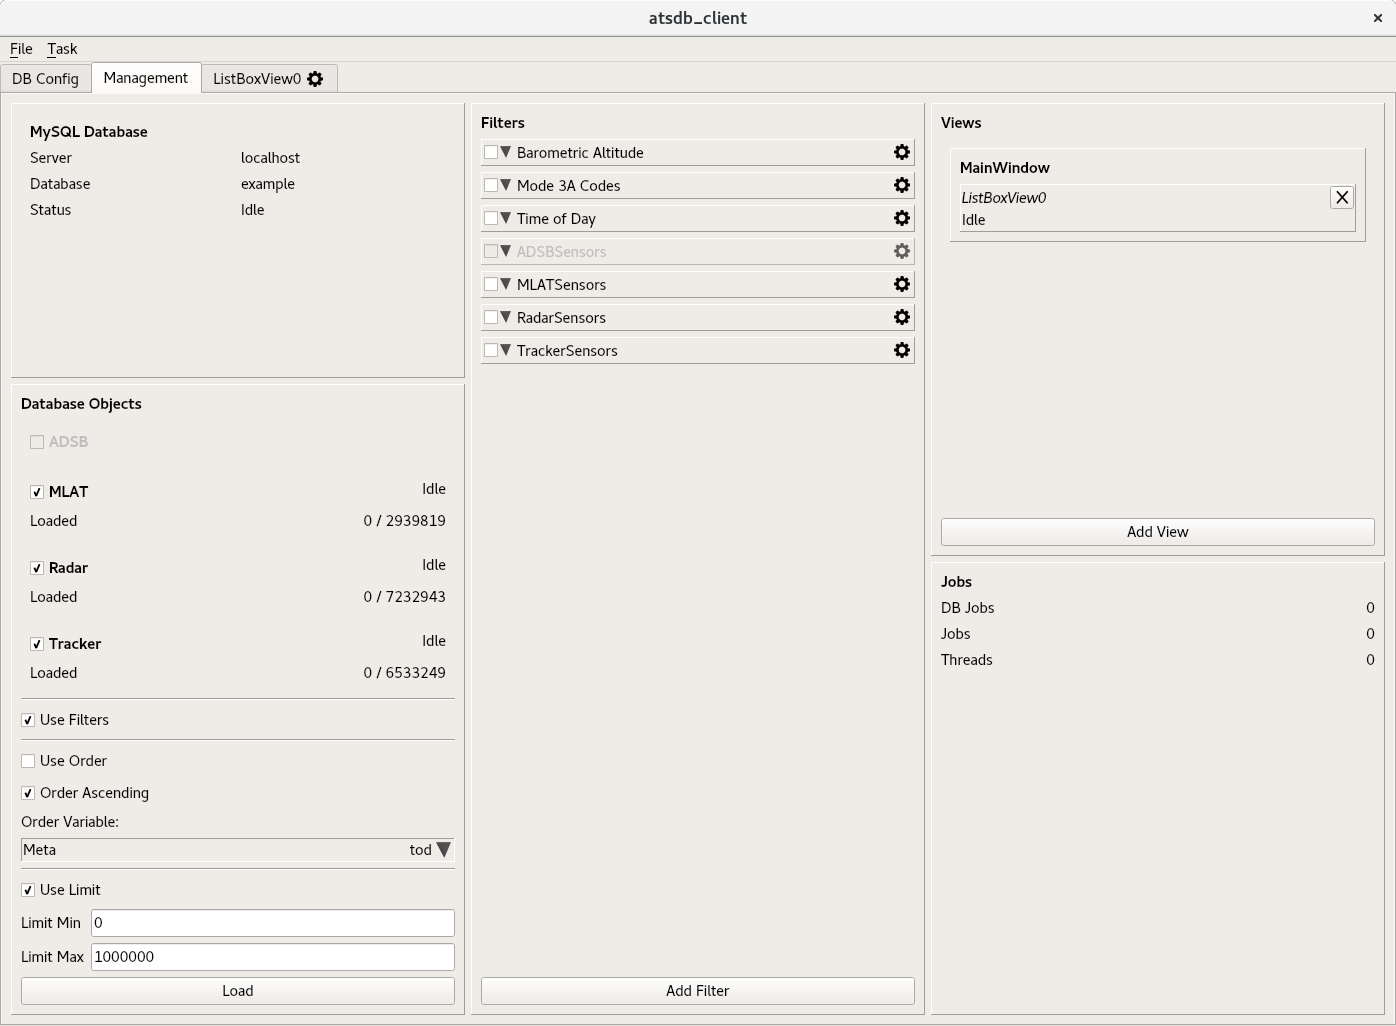
\includegraphics[width=18cm]{../screenshots/management.png}
  \caption{Main management window}
  \label{fig:management}
\end{figure}

In the uppermost part, the current tab can be selected. The following tabs exist:

\begin{table}[h]
  \center
  \begin{tabular}{ | l | l |}
    \hline
    \textbf{Tab} & \textbf{Description} \\ \hline
    DB Config & Database configuration, used during startup \\ \hline
    Management & All elements to manage loading and inspection of data \\ \hline
    ... & Additional tabs with Views \\
    \hline
  \end{tabular}
  \caption{Main window tab list}
\end{table}

Located in the main window, a management tab exists.  It shows general database information, a list of database objects with loading functions, a filter system and so on.

\subsection{Database Information}

In this widget, general information about the database is given. 

\begin{figure}[H]
  \center
    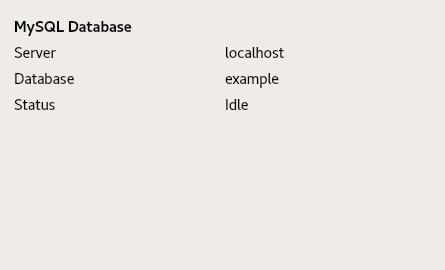
\includegraphics[width=8cm]{../screenshots/management_database.png}
  \caption{Management: Database Information}
  \label{fig:management_database}
\end{figure}

This also includes the working status, which can be:

\begin{itemize}
 \item Idle: Nothing to do at the moment
 \item Working: Database read/write in progress
\end{itemize}

\subsection{Database Objects}
\label{sec:management_dbos}

In this widget, information about the DBO's, the loaded dataset, and the loading parameters are given.

\begin{figure}[H]
  \center
    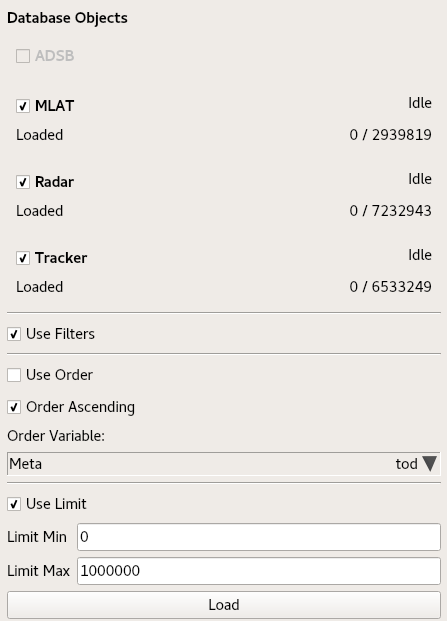
\includegraphics[width=8cm]{../screenshots/management_dbos.png}
  \caption{Management: Database Objects}
  \label{fig:management_objects}
\end{figure}

Each existing DBO is listed, and active ones have the following items:

\begin{itemize}
 \item Name checkbox: Defines whether data from this DBO should be loaded
 \item Loading status information
  \begin{itemize}
  \item Idle: Nothing to do at the moment
  \item Loading: DBO read/write in progress
  \end{itemize}
 \item Loaded data size: Number of loaded items / Number of existing items
\end{itemize}

If a DBO exists, but has no data in the database, it is shown as inactive (greyed out, like ADSB in the screenshot).\\

Additionally, parameters which configure the loading process exist:

\begin{itemize}
 \item ``Use Filters'' checkbox: Whether filtering should be performed
 \item ``Use order'' checkbox: Whether the dataset should be ordered by a DBO variable
 \item ``Use Ascending`` checkbox: If ordered, defines if it should be ascending or descending
 \item ''Order Variable`` selection: If ordered, what variable should be used
 \item ''Use Limit`` checkbox: If the data size should be limited
 \item ''Limit Min``: If limited, the data set will start at the n-th index given here. If 0, it will be loaded from the beginning, if e.g. 100, the first 100 entries will be skipped and the 101st entry will be the first in the dataset.
\item ''Limit Max'': If limited, the number given here will be the number of loaded entries.
\end{itemize}

Using the ``Load'' button , a loading process using the current configuration is started.

\subsection{Filters}

\begin{figure}[H]
  \center
    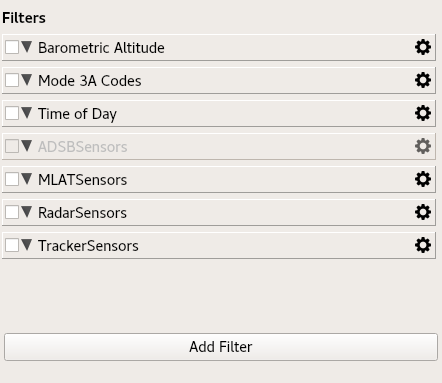
\includegraphics[width=8cm]{../screenshots/management_filters.png}
  \caption{Management: Filters}
  \label{fig:management_filters}
\end{figure}

Each filter consists of a checkbox, defining if a filter is active (contributes to the search query), a triangle-button (to show/hide the filter configuration elements), a unique name, and a manage button (activates a context menu). At the bottom an 'Add filter' button exists, which can be used to add new filters. \\

Please \textbf{note} that the filter configuration will be saved at program shutdown, which is also true for new
filters.   At  startup,  all  filters  from  the  configuration  are  generated  and  restored  to  their  previous  state. However, when the database was changed (usage of different data source), all filters are reset to an initial
state (since their previous configuration may be senseless). \\

Please also \textbf{note} that active filters, at the moment, are always combined with a logical AND. Therefore,
when  two  filters  are  active,  only  the  intersection  of  data  which  both  filters  allow  is  loaded.   A  logical combination of filters using an OR operation is planned, but was not implemented yet.

\subsubsection{Sensor Filters}
For each DBO with a sensor list, a sensor filter is generated which can not be edited or deleted.  For each
sensor a checkbox exists, which is only active if the sensor was active in the database.  If checked, the
data generated by the sensor is loaded, and vice versa.

\subsubsection{Custom filters}
A  custom  filter  does  not  differ  in  general  usage,  but  the  inner  workings  are  different.   Also,  it  can  be generated using the 'Add filter' button. It can also be reset (to the original values) edited and deleted using
the manage button. \\
A custom filter consists of one or more filter conditions.  Such a condition involves a DBO (or meta) variable, an operator, and a value.  When active, the filter restricts all loaded DBO data to be fullfill all filter conditions.
As an example, the ``Time of Day'' filter limits the loaded data to a specific time window, to load only time slices of the dataset.  The ``Mode 3A Codes`` filter restricts to a list of (comma-separated) mode 3/A codes, to single out specific flights. \\

For more information about filtering, please refer to Section \nameref{sec:filtering}.

\subsection{Views}

\begin{figure}[H]
  \center
    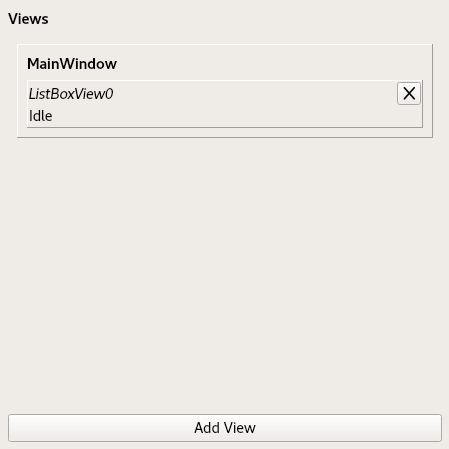
\includegraphics[width=8cm]{../screenshots/management_views.png}
  \caption{Management: Views}
  \label{fig:management_views}
\end{figure}

This element allows generation and management of all active Views and windows. Each View is contained
in a tab within a parent window.  At startup, only the main window exists ('MainWindow'), which also holds
the management tab. If the main window is closed, the ATSDB client shuts down. New Views can be added using the 'Add View' button, which opens a pull-down menu. Each View can either be added to the main window ('MainWindow') or into a new window. When added, a new tab exists in the containing window, and controlling elements are added for any new
windows or views. \\

Currently, only the Listbox View exist, for more information about this View, please refer to Section \nameref{sec:listbox_view}.\\

New Views can be added either to currently existing windows as new tabs, or to a newly opened window. A window can be closed either by the close button in the window decoration, which discards all contained Views within the window.  To delete a single View, one can use the close button in the GUI, which frees up all its allocated resources. Each View adds its required variables to the loading list for the database.  During a loading process, the loading status  of a View is shown in the management tab.\\

For more information about Views, please refer to Section \nameref{sec:inspection}.

\subsection{Jobs}

The ATSDB framework supports multi-threading. A number of processing steps (''Jobs``) can be exectuted on a number of parallel threads. Since multi-threading on a database creates limited benefit, only one thread is used specifically for database jobs. All non-database jobs are exectuted on a dynamic number of other threads, which are increased/decreased in number depending on the application's needs. 

\begin{figure}[H]
  \center
    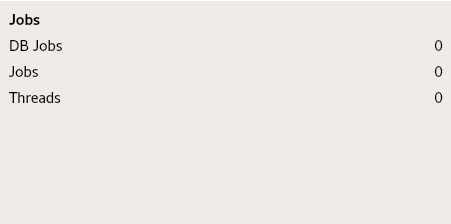
\includegraphics[width=8cm]{../screenshots/management_jobs.png}
  \caption{Management: Jobs}
  \label{fig:management_jobs}
\end{figure}

In the Job element the number of database jobs is listed under ''DB Jobs``, the number of other Jobs is listed under ''Jobs``. The number of active processing threads is listed under ''Threads``.

\section{Filtering}
\label{sec:filtering}

\subsection{Adding a New Filter}
When clicking the 'Add filter' button, a dialog is opened.

\begin{figure}[H]
  \center
    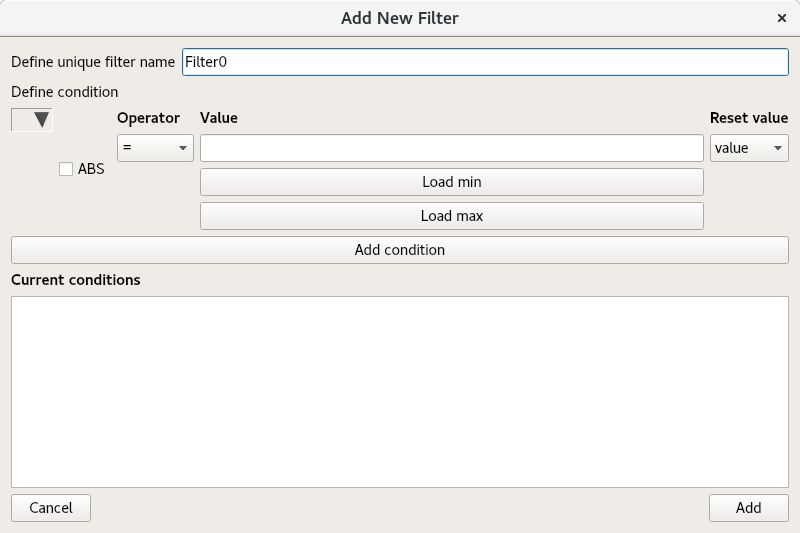
\includegraphics[width=14cm]{../screenshots/filter_add.png}
  \caption{Adding a filter}
  \label{fig:filter_add}
\end{figure}

First, one has to give the filter a new (unique) name. Then, conditions have to be defined and added. A condition consists of a DBO variable, an operator, a value, and a reset value. \\

When the triangular button is clicked, a sub-menu is opened, where one can choose a DBO variable. The selected variable restricts data of all DBOs if it is of type 'Meta', or just data from one DBO if it is not.Additionally, the mathematical operator 'ABS' can be selected. If so, not the value of the variable but the absolute value of the variable is used: 'ABS(var)>value' is equivalent to 'var>value OR var<-value'. \\

An operator can be chosen with the drop-down menu, the supplied operators are common SQL operators.

\begin{table}[H]
  \center
  \begin{tabular}{ | l | l |}
    \hline
    \textbf{Operator} & \textbf{Description} \\ \hline
    = & Equal \\ \hline
    != & Not equal \\ \hline
    > & Greater than \\ \hline
    >= & Greater than or equal \\ \hline
    < & Less than \\ \hline
    <= & Less than or equal \\ \hline
    IN & Matches a value in a list \\ \hline
    LIKE & Pattern matching with \% and \_ \\ \hline
    IS & Value NULL: No value exists \\ \hline
    IS NOT & Value NULL: Value exists \\
    \hline
  \end{tabular}
  \caption{SQL operators}
\end{table}

In the 'Value' field one can set a value manually, or load the minimum or maximum values of the selected DBO variable from the database using the 'Load min'/'Load max' buttons . A reset value also has to be supplied, which can be the chosen value or a minimum/maximum value set from the database.  Whenever a database different from the previous one is opened, all filters are reset, since previous values may have become invalid.\\

After a condition is defined, it has to be added using the 'Add condition' button. Existing conditions are
shown in the 'Current conditions' list. Please note that added conditions can not be removed in this dialog,
but have to be removed as described in the Section \nameref{sec:filter_editing}.

\begin{figure}[H]
  \center
    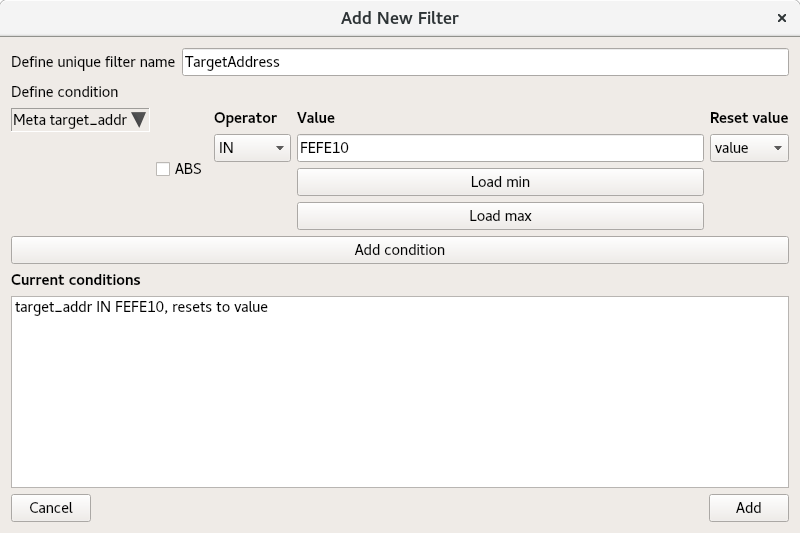
\includegraphics[width=14cm]{../screenshots/filter_add2.png}
  \caption{Filled out filter dialog}
  \label{fig:filter_add2}
\end{figure}

Now the described process can be repeated until a usable filter emerges, which is added using the 'Add'
button. The process of adding a new filter can be canceled by using the 'Cancel' button, which discards all
settings. When added, a new filter shows up immediately in the filter list and is saved to the configuration
for persistence.

\begin{figure}[H]
  \center
    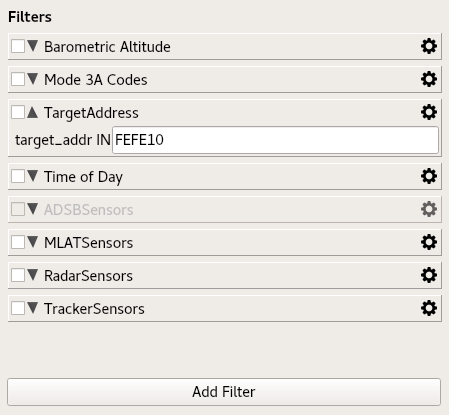
\includegraphics[width=8cm]{../screenshots/filter_add3.png}
  \caption{Filter added}
  \label{fig:filter_add3}
\end{figure}

\subsection{Editing a Filter}
\label{sec:filter_editing}

Currently, filter editing has been disabled and will be added at a later version.

%A filter can be reset (load reset values), edited or deleted.  When clicking on the manage button, a context menu appears. Please select the appropriate action, for editing select 'Edit'.

%(image here)

%When the 'Filter name' field is edited, its name is changed.  A new condition can be added using the
%'Define condition' elements, in the same manner as in the 'New filter' process. All existing conditions are
%shown at the bottom in rows.  Each condition can be deleted using the delete button, or changed using the elements in the appropriate row.
%All changes are immediately propagated to the filter in the Management tab.  When done, the window
%can be closed using the 'Close' button on the lower right.

\section{Tasks}
\label{sec:tasks}

Since in SASS-C Verif radar plot coordinates are not given as latitude/longitude, which are the main coordinates for all processing in ATSDB, optionally these coordinates can be re-calculated and set in the database using the ''Calculate Radar Plot Position`` Task.

\subsection{Calculate Radar Plot Position}
To execute this task select ''Task``->  ''Calculate Radar Plot Position` in the top menu bar.

\begin{figure}[H]
  \center
    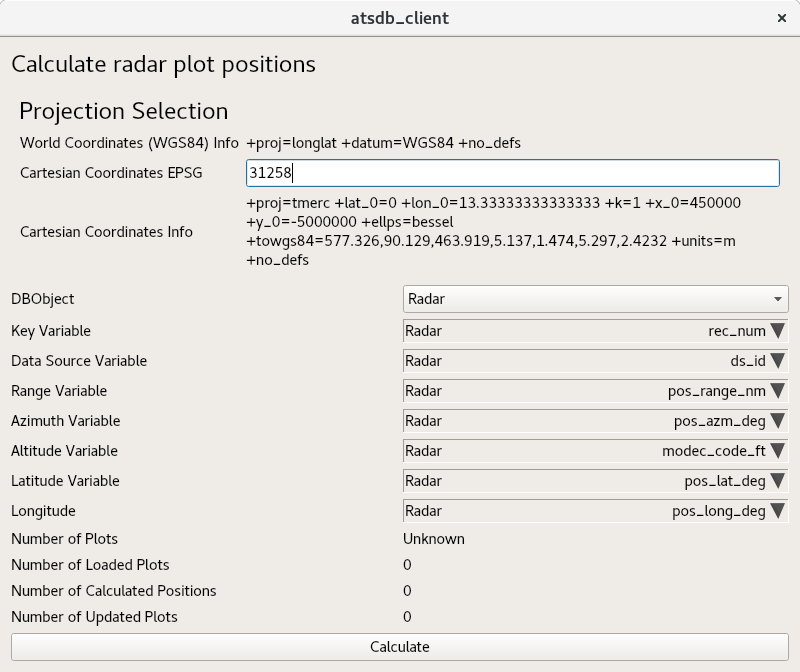
\includegraphics[width=14cm]{../screenshots/task_calc_radar.png}
  \caption{Calculate radar plot position task}
  \label{fig:task_calc_radar}
\end{figure}

The EPSG code for the projection has to be chosen according to your needs, please refer to \url{http://spatialreference.org/ref/epsg/} for a list of possible codes.

The WGS84 latitude/longitude coordinates are then calculated using the radar positions in the database, the range and the azimuth. Press ``Calculate'' to start the calculation process, which will take a few minutes depending on the data size. \\

Please \textbf{note} that currently the various ``Number of'' labels are not set correctly, and no status indication exists. This will be fixed in a later version. \\

Messages like these will be printed in the text console, the last one indicates completion of the task:

\begin{verbatim}
...
[INFO] RadarPlotPositionCalculatorTask: loadingDoneSlot: starting calculation
[INFO] RadarPlotPositionCalculatorTask: loadingDoneSlot: writing update_buffer
[INFO] RadarPlotPositionCalculatorTask: loadingDoneSlot: update_buffer size 7230527
[INFO] RadarPlotPositionCalculatorTask: loadingDoneSlot: end
[INFO] UpdateBufferDBJob: run: start
[INFO] UpdateBufferDBJob: run: writing object Radar key rec_num size 7230527
[INFO] BufferWriter: update: buffer size 7230527 into table sd_radar
[INFO] SQLGenerator: createDBUpdateStringBind: idvar name REC_NUM
[INFO] BufferWriter: update: preparing bind statement
[INFO] BufferWriter: update: starting inserts
[INFO] BufferWriter: update: bind transactions cnt 0
[INFO] BufferWriter: update: bind transactions cnt 100000
...
[INFO] BufferWriter: update: bind transactions cnt 7200000
[INFO] BufferWriter: update: ending bind transactions
UpdateBufferDBJob: run: buffer write done (411.33 s).
\end{verbatim}

After running this task once (per database), the radar plots also have a set latitude/longitude. This task can be re-run with different projections if wanted.

\section{Inspection}
\label{sec:inspection}

\subsection{Listbox View}
\label{sec:listbox_view}
A Listbox View displays the DBO records as text in tables, to allow full data inspection. When started, it presents itself in the following manner.

\begin{figure}[H]
    \hspace*{-2cm}
    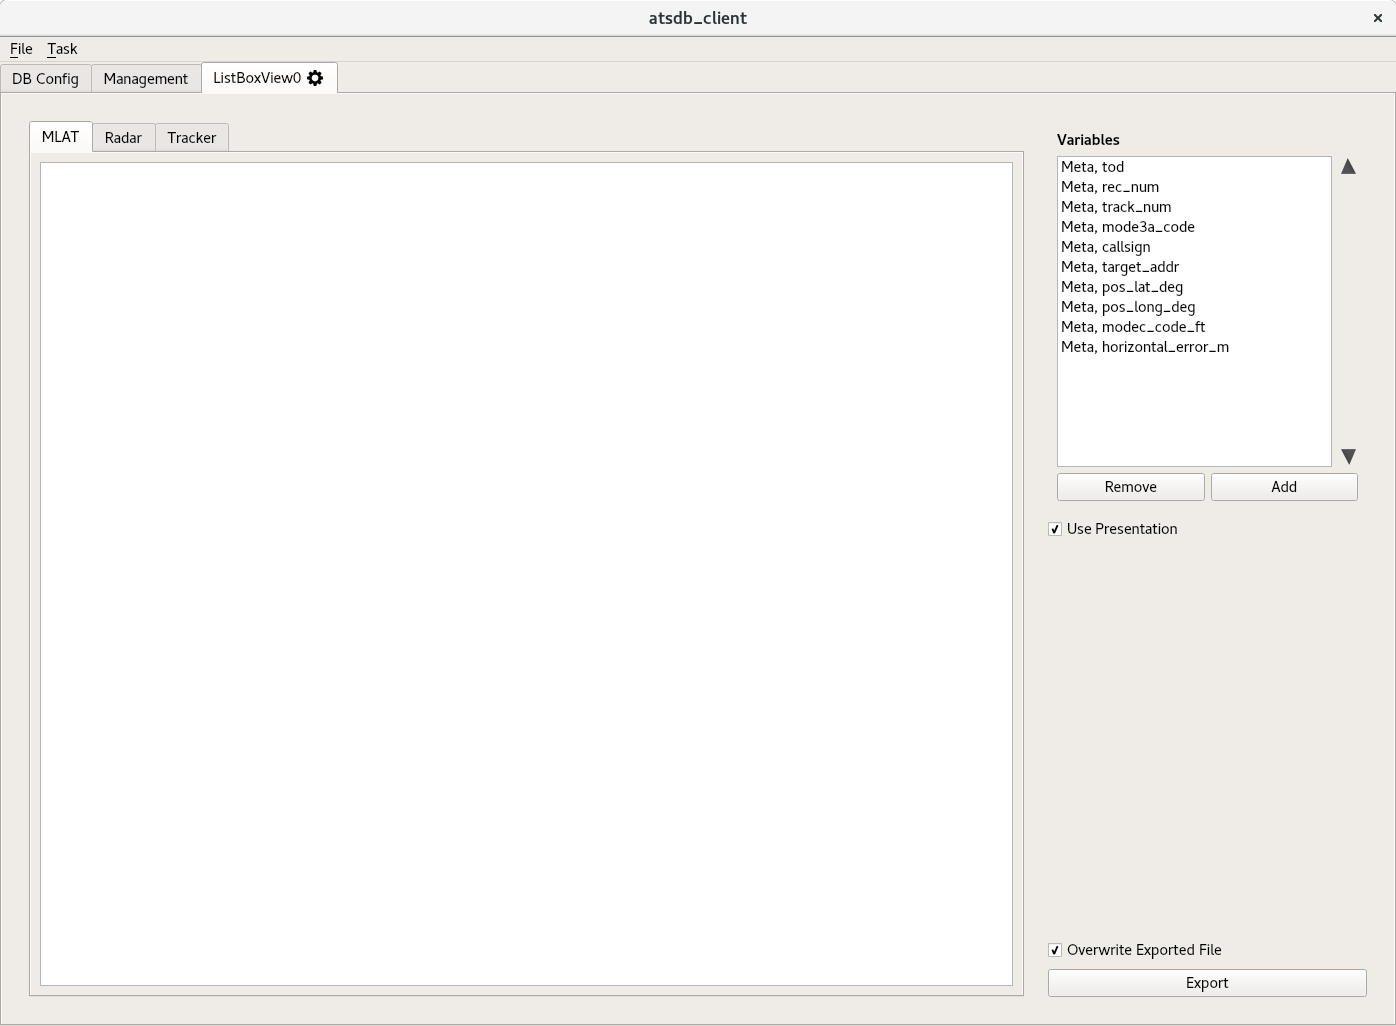
\includegraphics[width=18cm]{../screenshots/listbox_start.png}
  \caption{Listbox View startup}
  \label{fig:listbox_start}
\end{figure}

On the left side, a number of tabs exist for each active DBO, each of which contains a table. On the right side, a configuration area exists. A number of variables is displayed in the 'Variables' list. One can change the order, remove and add variables to be inspected. \\

To limit, order based on a variable or load the dataset, the mechanism described in Section \nameref{sec:management_dbos} can be used. To filter the dataset, the mechanism described in Section \nameref{sec:filtering} can be used.

\begin{figure}[H]
    \hspace*{-2cm}
    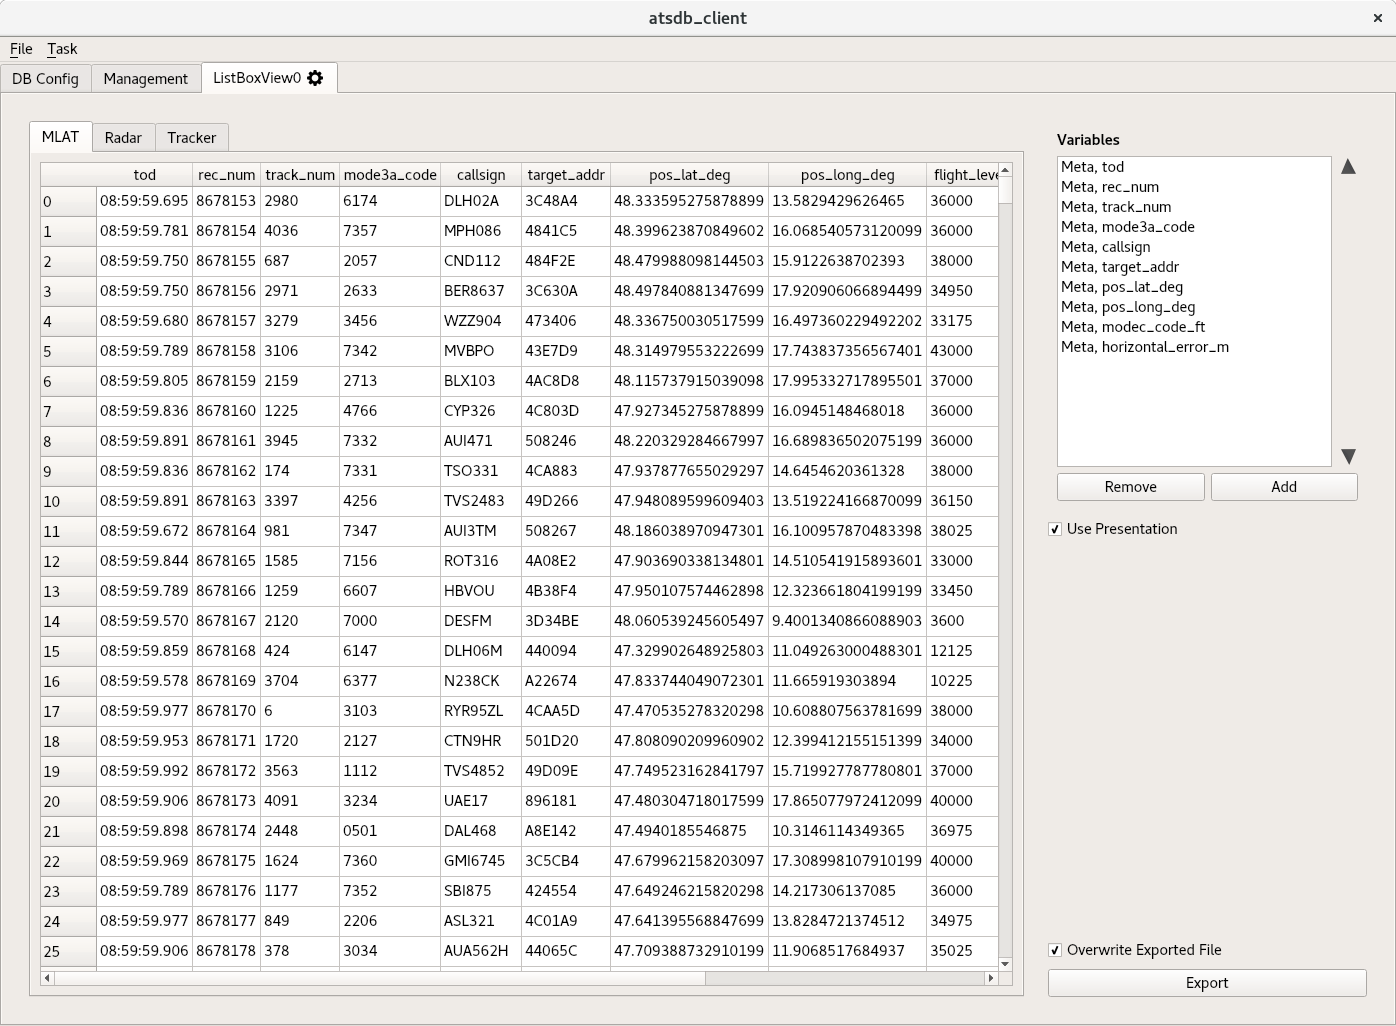
\includegraphics[width=18cm]{../screenshots/listbox_loaded.png}
  \caption{Listbox View after loading}
  \label{fig:listbox_load}
\end{figure}

Once updated, the tables are filled with text representing the values of the DBO variables.  If a value is undefined its cell is empy. \\

Please \textbf{note} that since some variable might only exist in some DBOs, the number of columns for different DBOs may differ.

\subsubsection{Variable List}
All DBO variables which are loaded from the database are shown in the 'Variables' list. This list is ordered,
and like all configuration elements persistent. Ordering can be changed by selecting (clicking on) a variable
and using the up/down triangle buttons.
When pressing the 'Remove' button, a selected variable is removed.  Pressing the 'Add' button allows
appending a variable to the list using a context-menu.

\subsubsection{Use Presentation}
When this checkbox is checked, the so called presentation mode is used. In the database, the variables might have different units or a data representation which is not easy to read. For this purpose, a presentation mode was introduced to e.g. show a Mode A code as octal, or a Time of Day not in seconds since midnight but in HH::MM:SS.SS format. When the ''Use Presentation`` checkbox is not checked, the original database values are presented (and exported).

\subsubsection{Exporting}

The data from the current DBO table can be exported to a comma-separated value (CSV) text file. 

When pressing the ''Export`` button, a dialog is opened.

\begin{figure}[H]
    \hspace*{-2cm}
    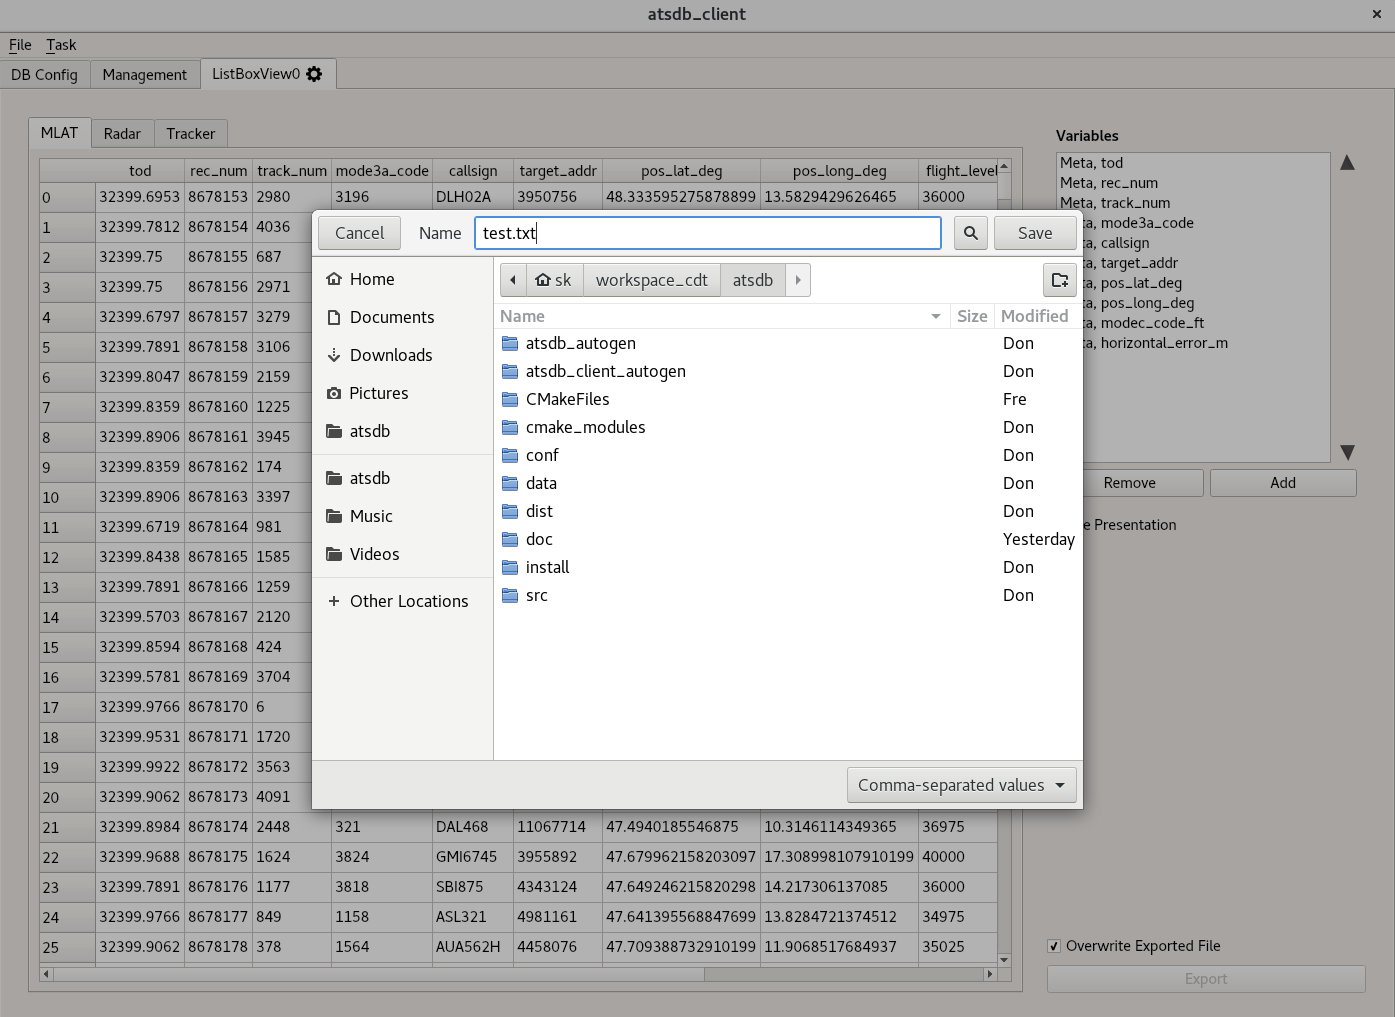
\includegraphics[width=18cm]{../screenshots/listbox_export.png}
  \caption{Listbox View export}
  \label{fig:listbox_export}
\end{figure}

Choose a filename, and press ''Save`` to save the data. If the ''Overwrite Exported File`` checkbox was checked, an existing file is automatically overwritten. Please \textbf{note} that exporting might take some time for larger datasets, and currently no status indication is given.\\
After export, a dialog is shown indicating that the export was completed.

\begin{figure}[H]
    \hspace*{-2cm}
    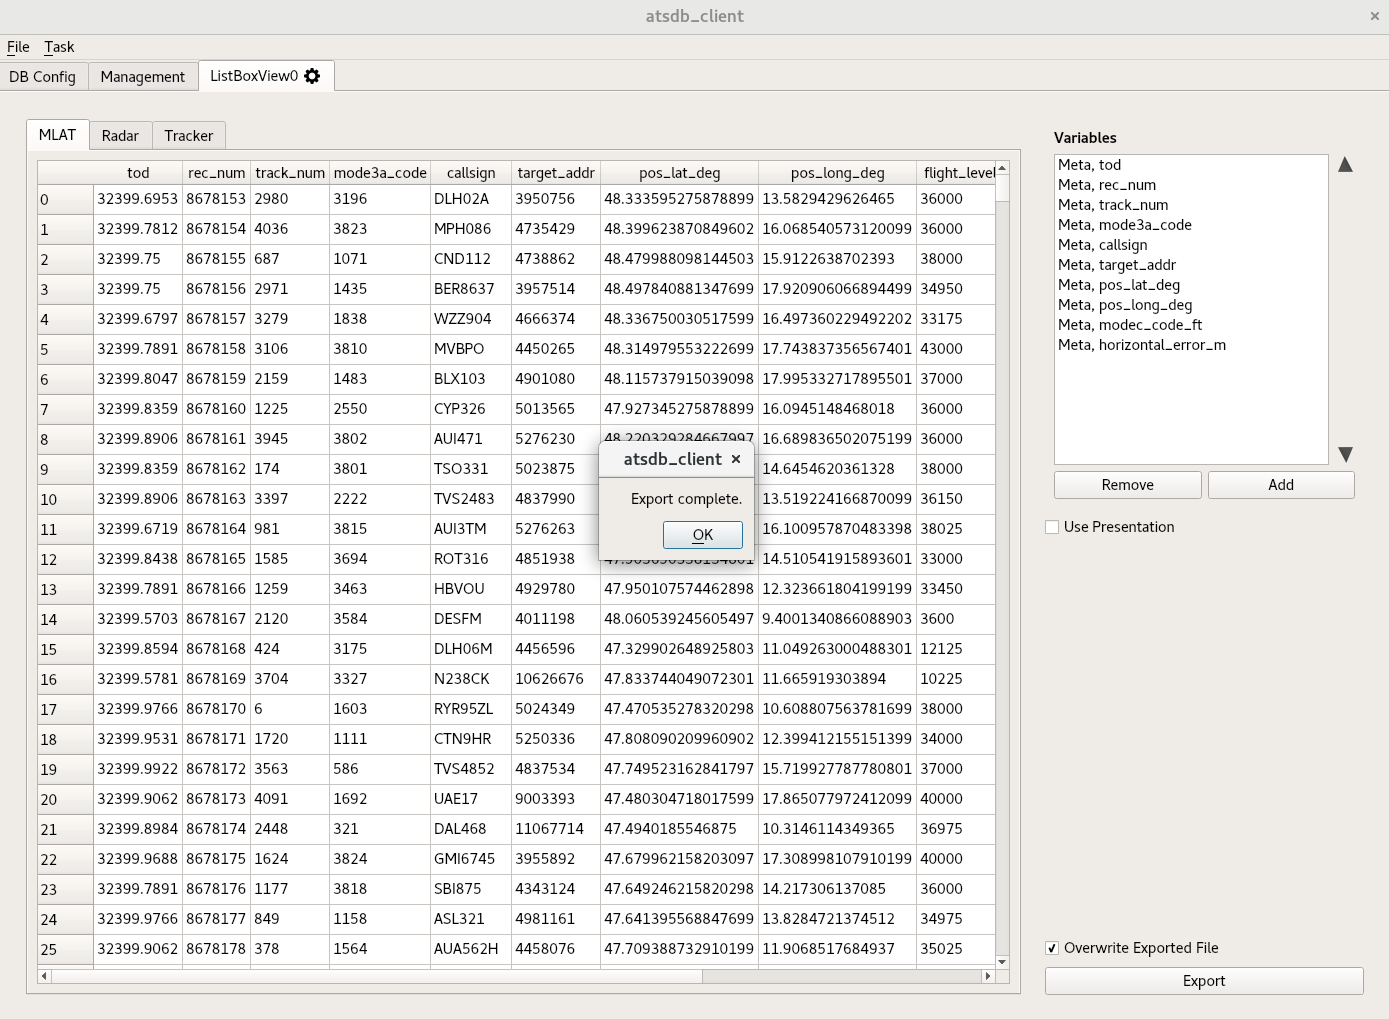
\includegraphics[width=18cm]{../screenshots/listbox_exported.png}
  \caption{Listbox View export done}
  \label{fig:listbox_exported}
\end{figure}

The exported file can be opened in any editor, or for example imported into LibreOffice Calc.

\begin{figure}[H]
    \hspace*{-2cm}
    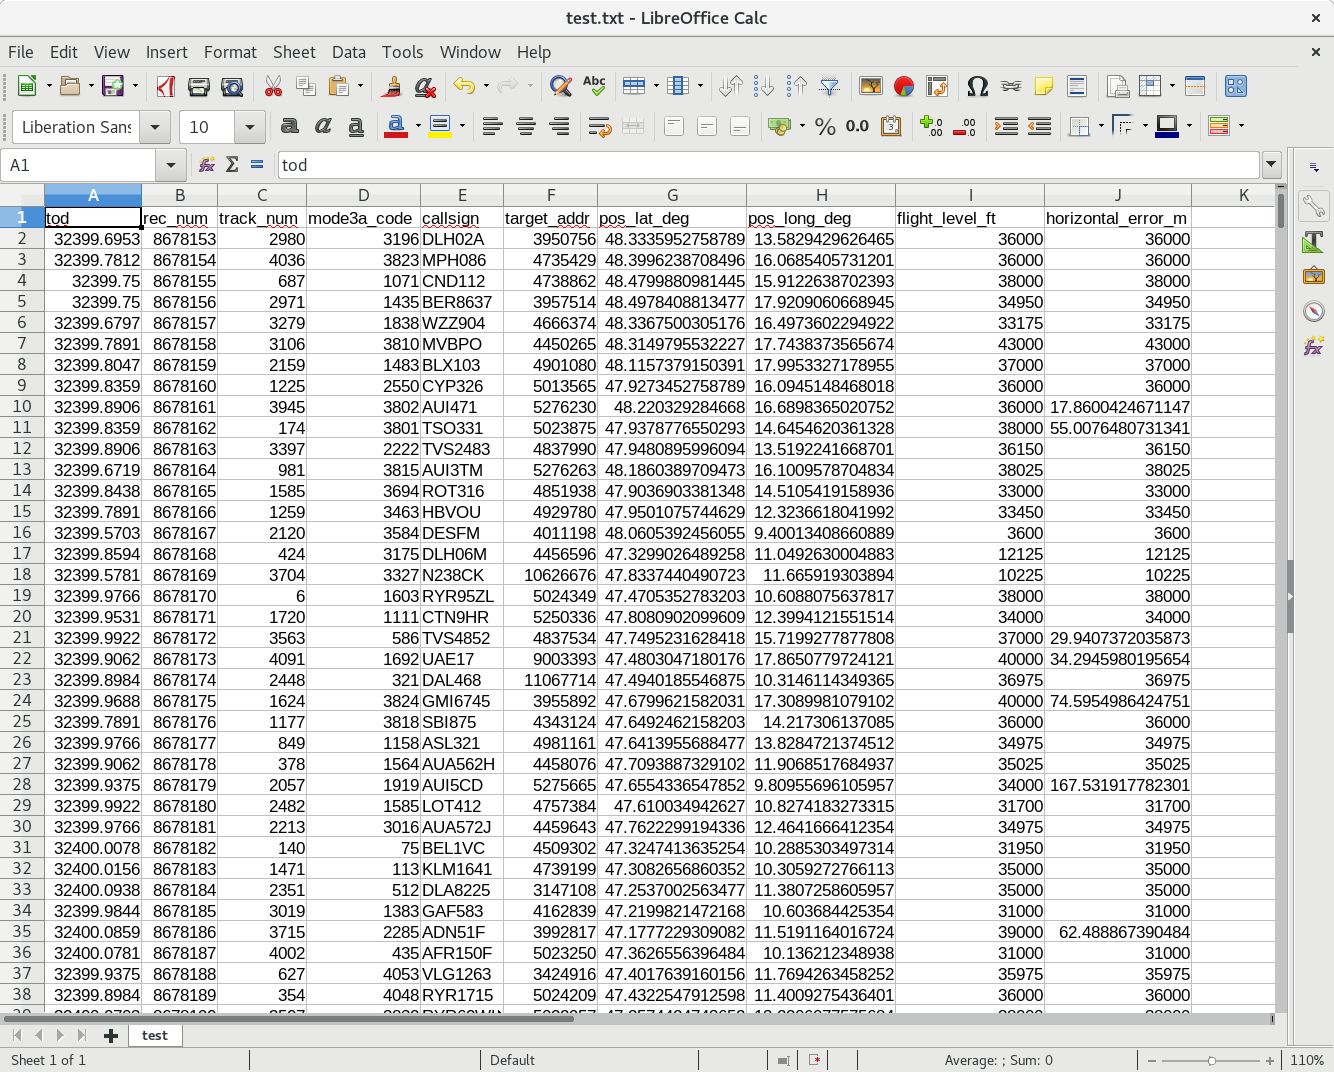
\includegraphics[width=18cm]{../screenshots/listbox_exported_calc.png}
  \caption{Listbox View export in LibreOffice Calc}
  \label{fig:listbox_export_calc}
\end{figure}

\subsection{OSG View}
\label{sec:osgview}

The OSG View allows a graphical representation of target reports from the Database Objects. After creation, it displays a world map in the map widget on the left, supported by a configuration panel on the right hand side.

\begin{figure}[H]
    \hspace*{-2cm}
    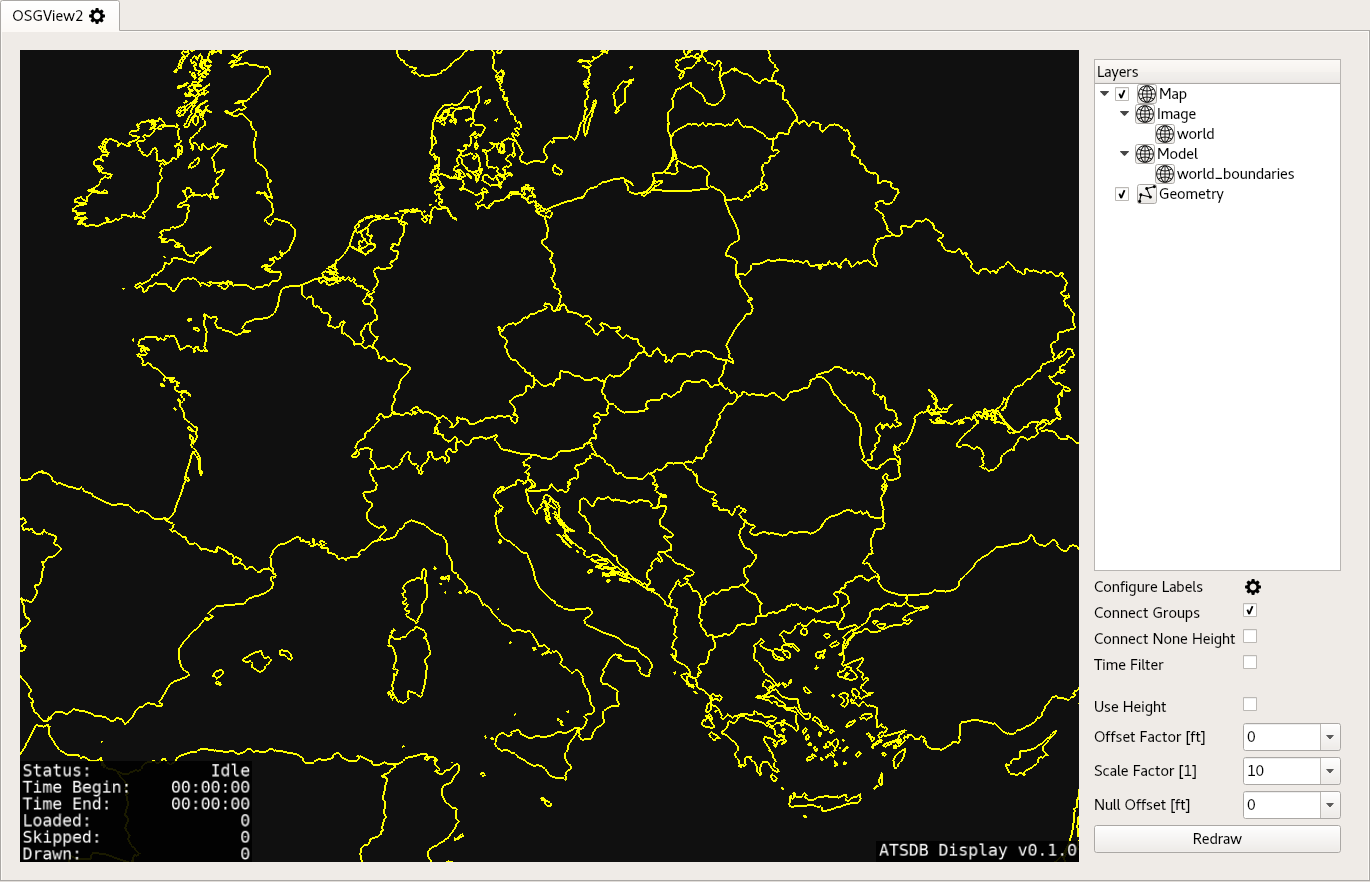
\includegraphics[width=18cm]{../screenshots/osgview_overview.png}
  \caption{OSG View overview}
  \label{fig:osgview_overview}
\end{figure}

The map window will automatically traverse to the medium location of the data in the current database.

\subsubsection{Map Widget}
\label{sec:osgview_map}

In the map widget, several mouse and key operations are supported. The following terms are used:

\begin{itemize}
 \item LMB: Left mouse button
 \item MMB: Middle mouse button
 \item RMB: Right mouse button
 \item CTRL: CTRL key
\end{itemize}

\begin{table}[H]
  \center
  \begin{tabular}{ | l | l | l |}
    \hline
    \textbf{Mouse Action} & \textbf{Key Action} &  \textbf{Description} \\ \hline
    Single click & - & - \\ \hline
    LMB click \& drag & - & Traverse map \\ \hline
    - & Arrows & Traverse map \\ \hline
    MMB click \& drag & - & Rotate map \\ \hline
    RMB click \& drag & - & Zoom map \\ \hline
    MMB scroll \& drag & - & Zoom map \\ \hline
    LMB double click & - & Zoom to clicked location \\ \hline
    RMB double click \& drag & - & Zoom away from clicked location \\ \hline
    - & Space bar & Return to home position \\ \hline
  \end{tabular}
  \caption{Map widget view operations}
\end{table}

Further operations are defined in section \ref{sec:osgview_map_operations}.

\subsubsection{Configuration Widget}
\label{sec:osgview_config}

In the configuration widget, several elements exist:

\begin{itemize}
 \item Layer widget: displays all currently existing layers
 \item Height widget: configures if and how height information is used
 \item Time filter: De/activates the time window filter
\end{itemize}

\subsubsection{Layer Widget}

In the layer widget, a tree view is given to configure the display of the existing elements. The following main tree elements are:
\begin{itemize}
 \item Map: Shows current map layers
 \item Geometry: Shows current DBO elements
\end{itemize}

\subsubsection{Changing the Background Map}

Please note that, while the default background map is supplied ATSDB, the other background map types are downloaded from public Internet sources and therefore require an Internet connection. They are then cached locally to facilitate faster access. \\

To change the background map, click the globe symbol {
\includegraphics[scale=0.05]{../../data/icons/globe.png} in Map Layer to access the map selection. The following maps are commonly available:

\begin{itemize}
 \item arcgis.earth
 \item minimal.earth
 \item openstreetmap.earth
 \item readymap.earth
 \item readymap-detailed.earth
\end{itemize}

The map loading and display in based on the osgEarth library (\url{http://osgearth.org/}), as are to map file definitions. The map which can be set using this dialog is simply a file list from the folder '~/.atsdb/data/maps'. So, changes can be made to the supplied ones or custom user maps can be added to this folder. \\
Please refer to \url{http://docs.osgearth.org/en/latest/references/earthfile.html} for a definition of an earth file.

\newpage
\paragraph{ArcGIS Map}

As supplied in the osgEarth example files, this map data is obtained from ArcGIS Online (\url{https://doc.arcgis.com/en/arcgis-online/reference/what-is-agol.htm}). It shows satellite imagery, supplied with elevation data from ReadyMap. 

\begin{figure}[H]
    \hspace*{-2cm}
    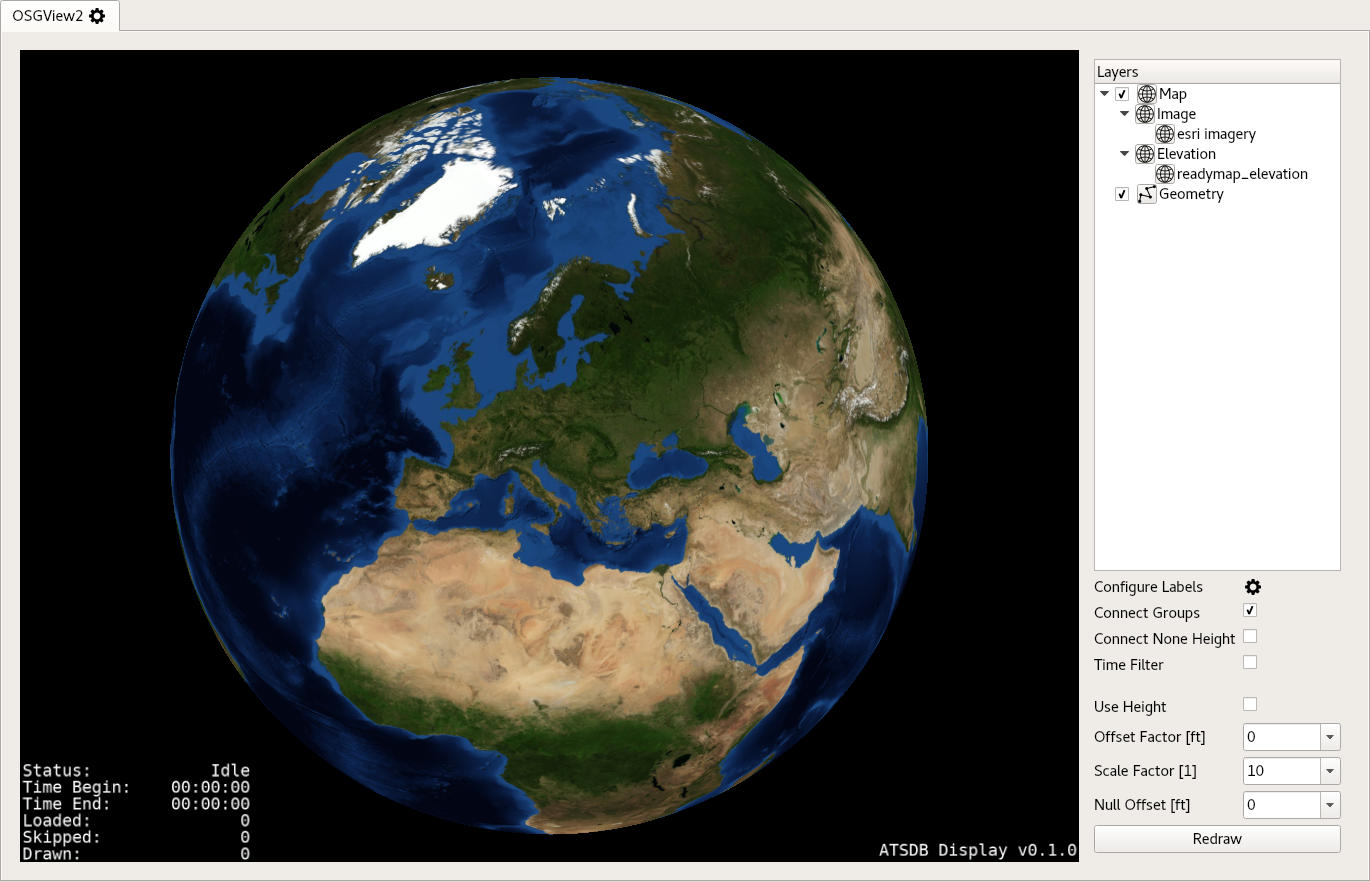
\includegraphics[width=18cm]{../screenshots/osgview_arcgis.png}
  \caption{OSG View Arcgis map}
\end{figure}

\newpage
\paragraph{Minimal Map}

This minimal map shows national borders based on an ESRI shapefile, provided by Bjorn Sandvik on \url{thematicmapping.org}.

\begin{figure}[H]
    \hspace*{-2cm}
    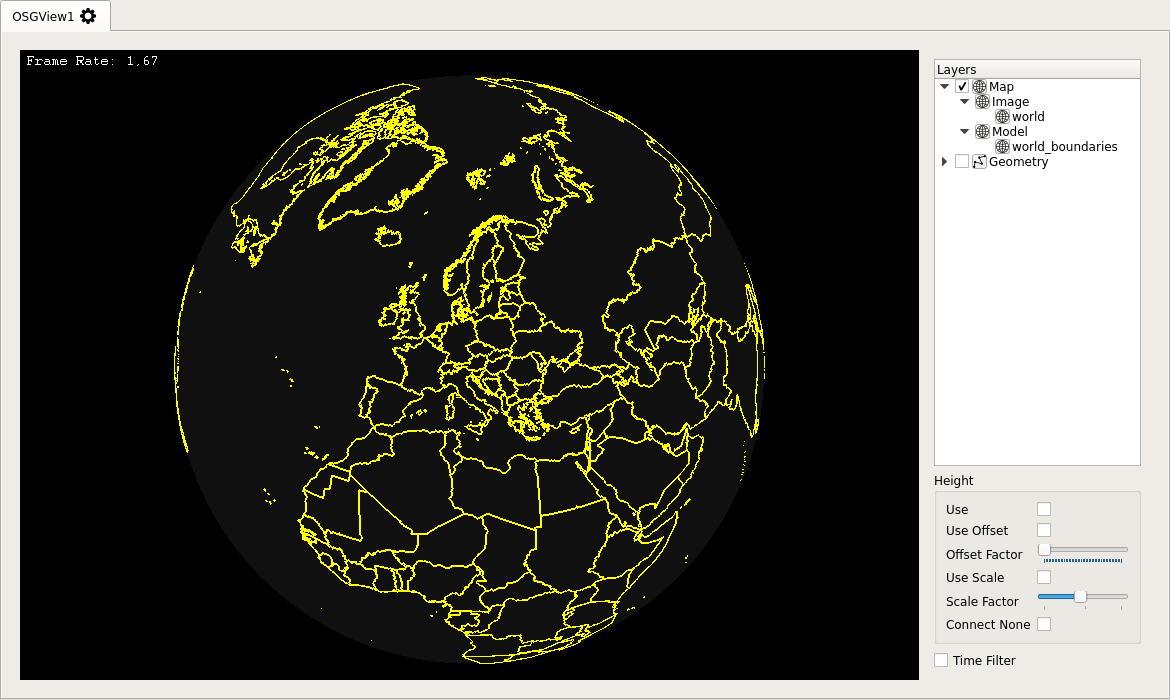
\includegraphics[width=18cm]{../screenshots/osgview_minimal.png}
  \caption{OSG View minimal map}
\end{figure}

\newpage
\paragraph{Open Street Map}

This very useful map shows map data from \url{https://www.openstreetmap.org/}.

\begin{figure}[H]
    \hspace*{-2cm}
    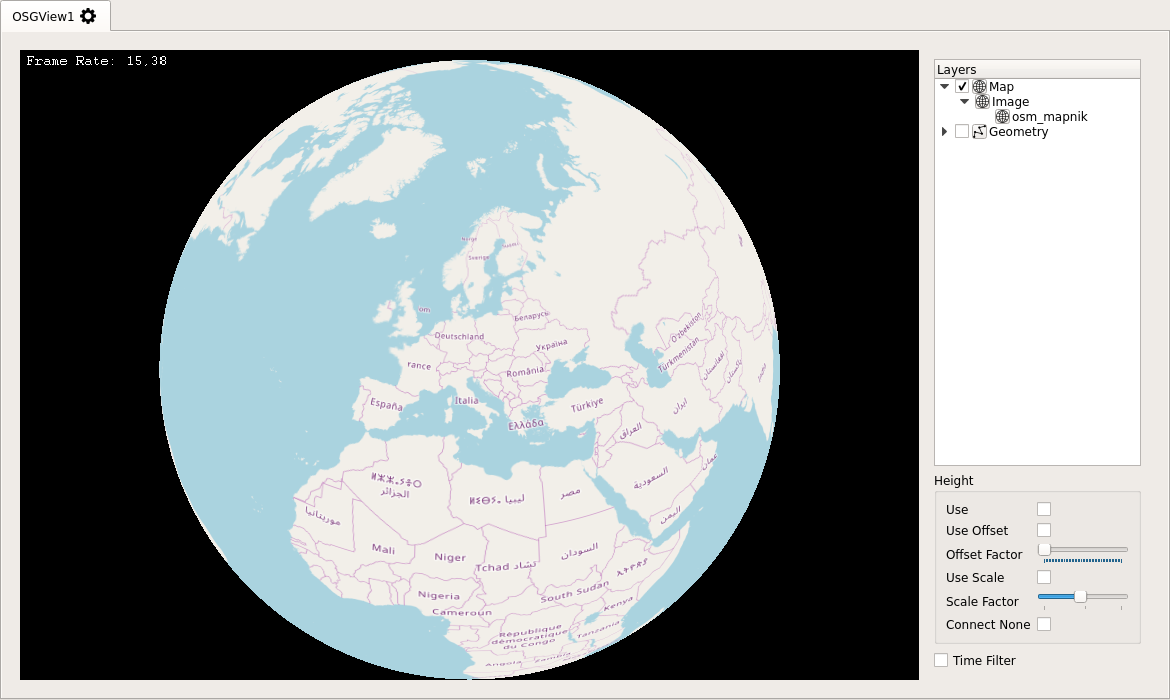
\includegraphics[width=18cm]{../screenshots/osgview_osm.png}
  \caption{OSG View OpenStreetMap}
\end{figure}

It is possible to zoom in to a very high level of detail, to even inspect airport layouts.

\begin{figure}[H]
    \hspace*{-2cm}
    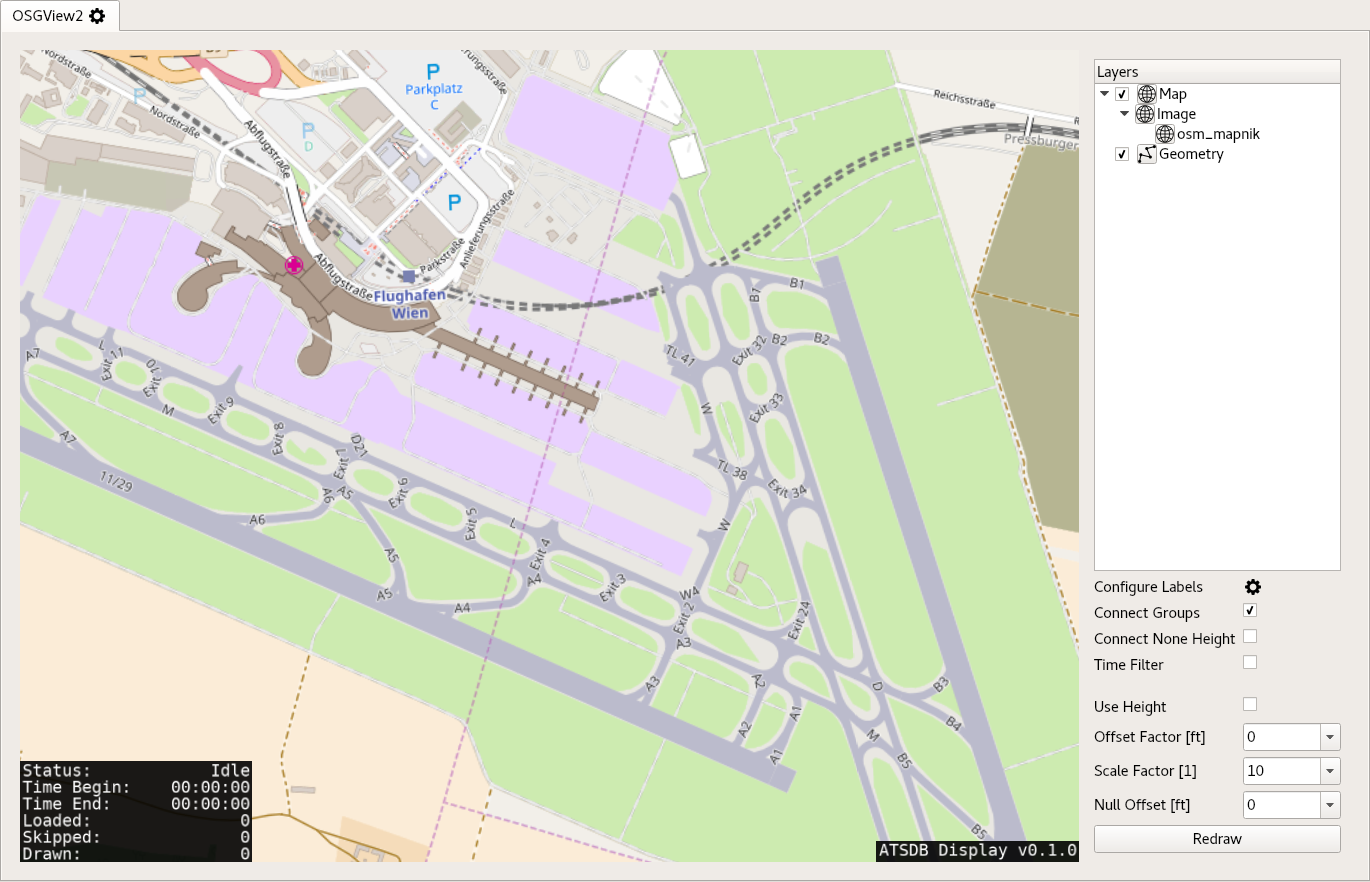
\includegraphics[width=18cm]{../screenshots/osgview_osm_vienna.png}
  \caption{OSG View OpenStreetMap Vienna Airport}
\end{figure}

\newpage
\paragraph{ReadyMap}

This map also shows satellite data, from \url{http://web.pelicanmapping.com/readymap-tiles/}. It includes an elevation layer, so ground elevation is observable.

\begin{figure}[H]
    \hspace*{-2cm}
    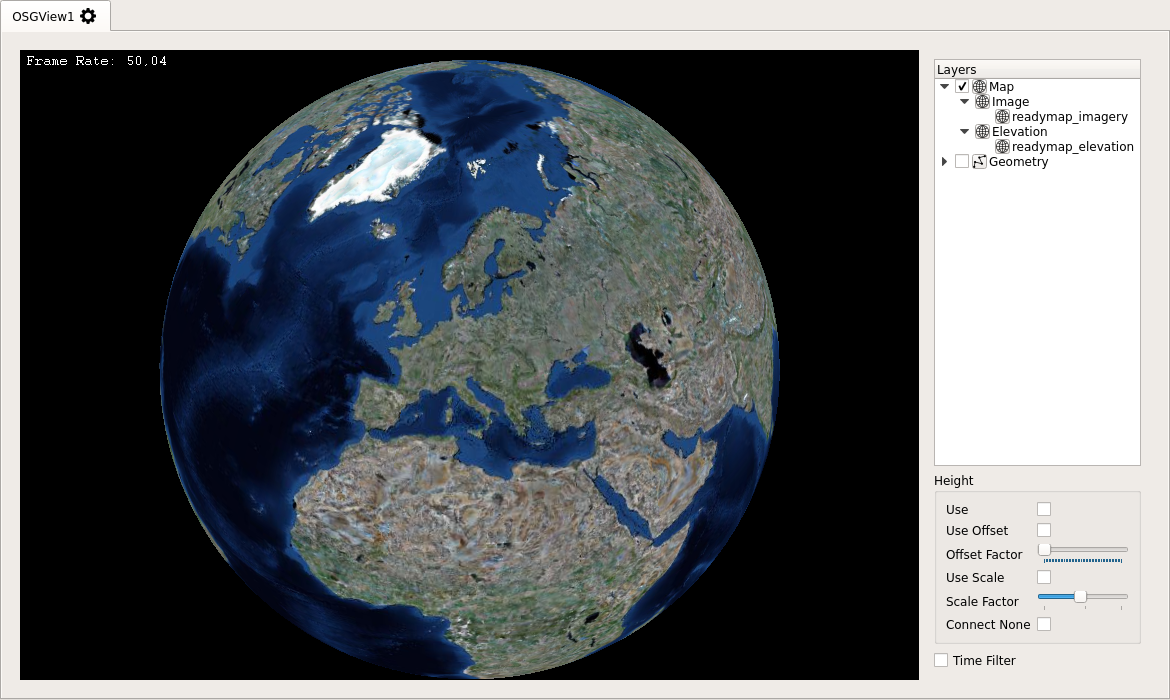
\includegraphics[width=18cm]{../screenshots/osgview_ready.png}
  \caption{OSG View ReadyMap}
\end{figure}


\paragraph{ReadyMap Detailed}

This map shows the same data as ReadyMap, but to a higher detail level.

\begin{figure}[H]
    \hspace*{-2cm}
    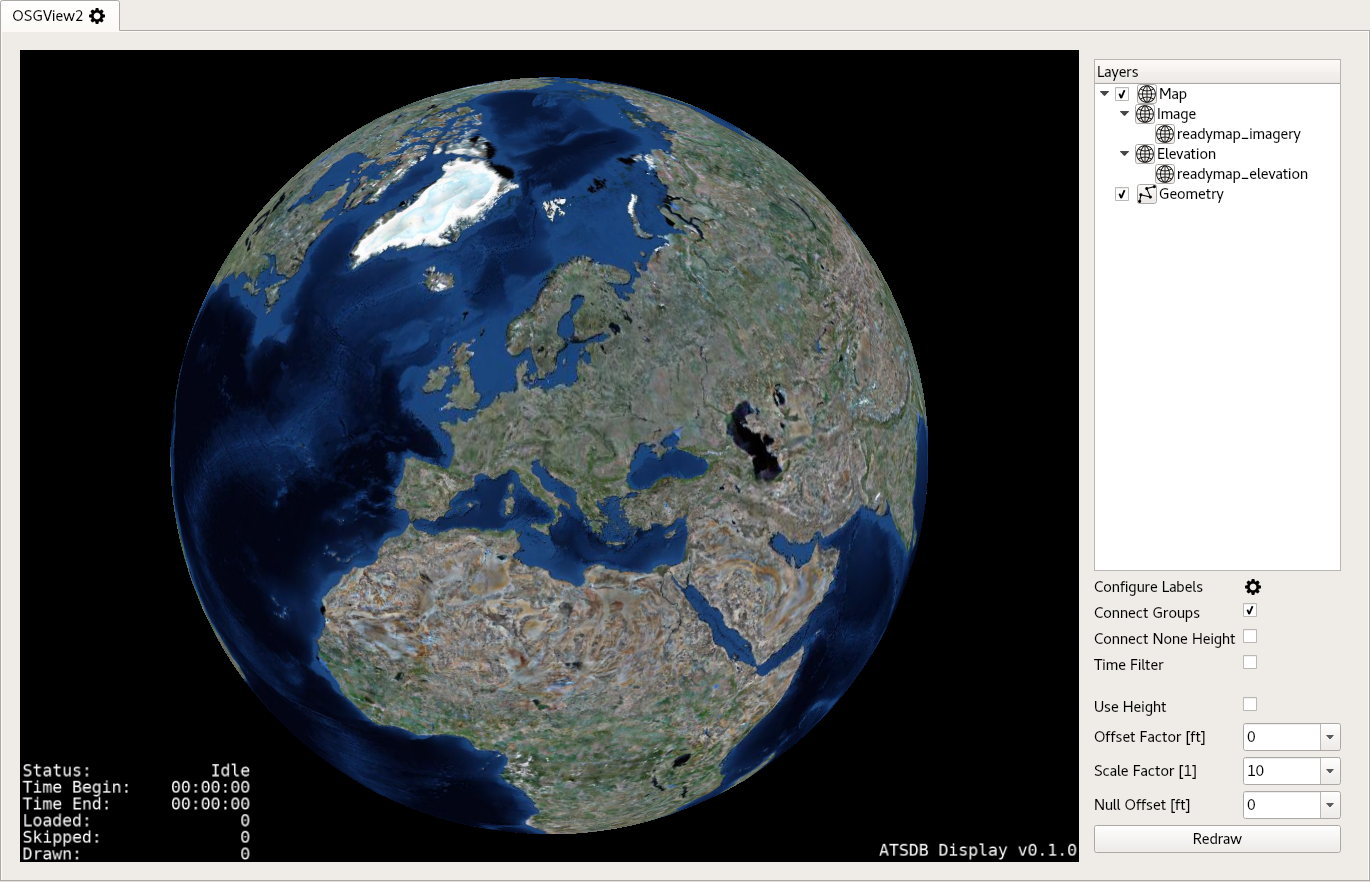
\includegraphics[width=18cm]{../screenshots/osgview_ready_detail.png}
  \caption{OSG View ReadyMap detailed}
\end{figure}


\begin{figure}[H]
    \hspace*{-2cm}
    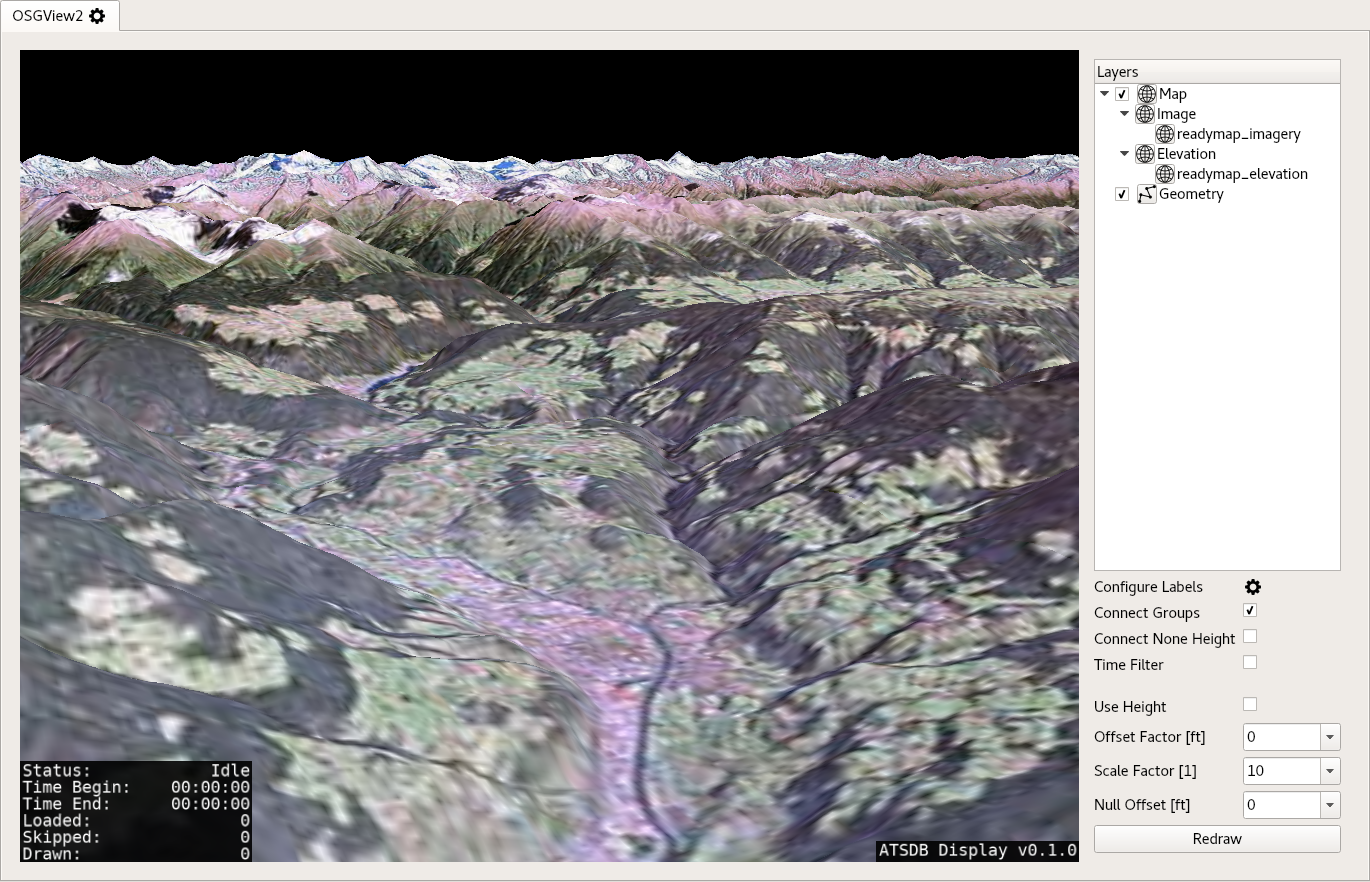
\includegraphics[width=18cm]{../screenshots/osgview_readymap_elav.png}
  \caption{OSG View ReadyMap detailed elevation}
\end{figure}


\subsubsection{Loading Data}
To load data, trigger a loading action from the Management widget. The data will be loaded as with the Listbox View, and displayed during the loading process. 

\begin{figure}[H]
    \hspace*{-2cm}
    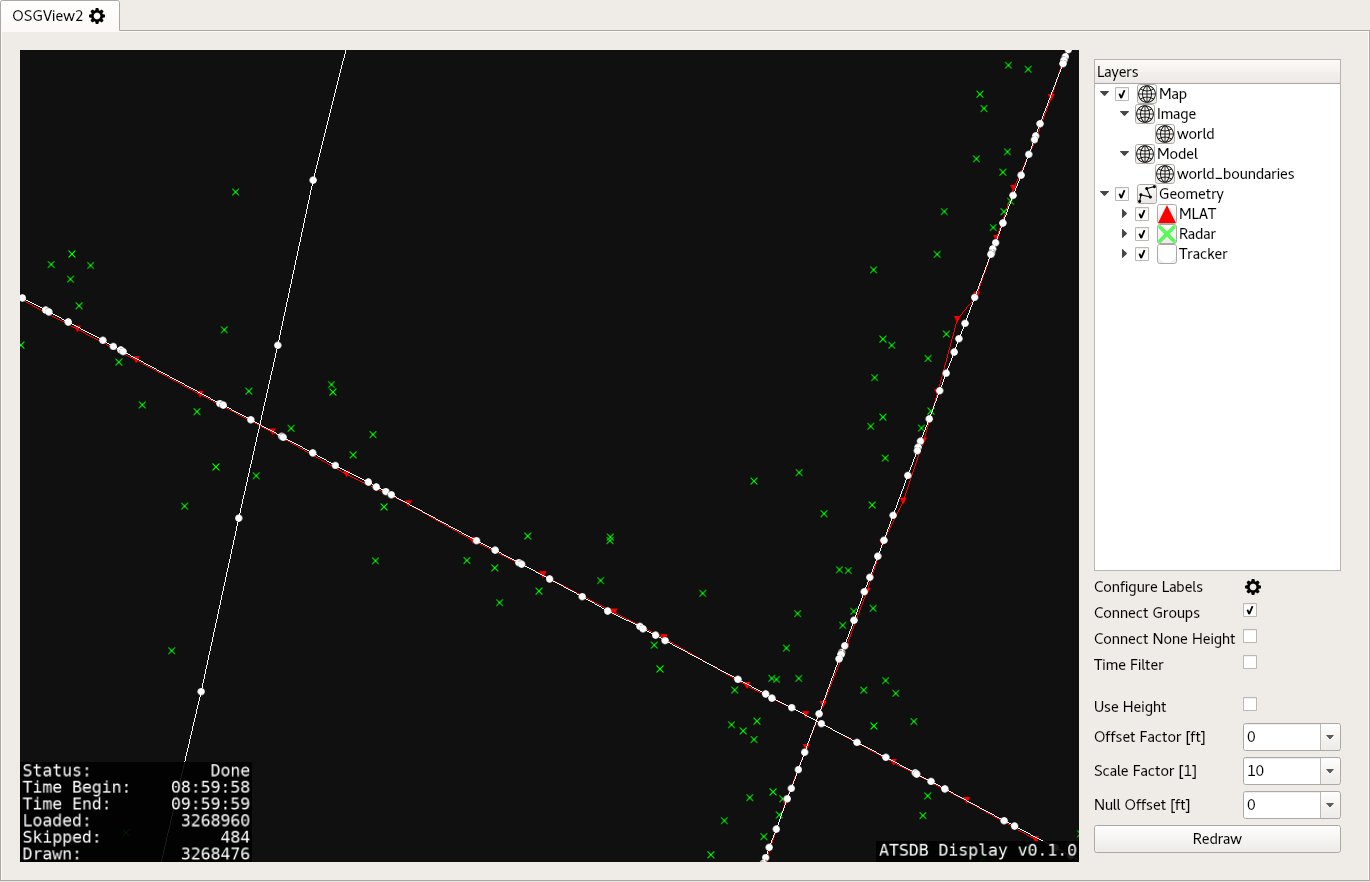
\includegraphics[width=18cm]{../screenshots/osgview_data.png}
  \caption{OSG View data display}
  \label{fig:osgview_data}
\end{figure}

Please note that since currently only an example dataset is used, until real surveillance data can be made available.

Now, the loaded data is displayed in the following manner: For each DBO, a list of sensors exist, which supply the shown target reports. In the Geometry layers, the data is grouped as follows: Database Object $\rightarrow$ Sensor $\rightarrow$ Group. \\

For each DBO, a default display configuration is set:

\begin{itemize}
 \item ADS-B: Blue square
 \item MLAT: Red triangle
 \item Radar: Green cross
 \item Tracker: White circle
\end{itemize}

A sensor is of course a defined data source, e.g. a specific radar. A group currently is defined by a track number, and is connected by lines. If no track number is defined, the data is put into the 'Unassociated' group and not connected by lines.

\subsubsection{Layer Operations}

In the Layers widget, a number of operations are possible for each tree item.

\begin{table}[H]
  \center
  \begin{tabular}{ | l | l | l |}
    \hline
    \textbf{Operation} & \textbf{Trigger} &  \textbf{Description} \\ \hline
    View sub-items & Triangle & Opens or closes view of the sub-items \\ \hline
    Display item & Checkbox & Enables or disables display of items (and all sub-items) \\ \hline
    Display context menu & Click on symbol & Opens the items context menu \\ \hline
  \end{tabular}
  \caption{Layer operations}
\end{table}

The context menu allows several actions to be performed on an item. If an item has sub-items, the same action will automatically be performed on the child items.

\begin{figure}[H]
    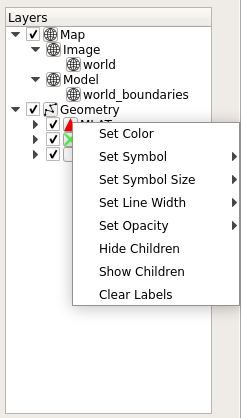
\includegraphics[width=5cm]{../screenshots/osgview_layer_context_menu.png}
  \caption{OSG View layer context menu}
\end{figure}

\begin{itemize}
 \item Set Color: Open colour dialog to set the items colour
 \item Set Symbol: Set the items symbol to one of the following values:
\begin{itemize}
 \item Cross
 \item Circle
 \item Square
 \item Triangle
\end{itemize}
 \item Set Symbol Size: Set the symbols size
 \item Set Line Width: Set the line width
 \item Set Opacity: Set the items opacity
 \item Hide children: Disable display off all children
 \item Show Children: Enable display of all children
 \item Clear Labels: Removes all labels
\end{itemize}

Please note that only the main Map item has a context menu, and only allows setting of map files and changing the opacity.

\subsubsection{Map Widget Data Operations}
\label{sec:osgview_map_operations}

Several data-related operations can be also performed in the map widget.

\begin{table}[H]
  \center
  \begin{tabular}{ | l | l | l |}
    \hline
    \textbf{Mouse Action} & \textbf{Key Action} &  \textbf{Description} \\ \hline
    LMB click & CTRL & Toggle label display of a single target report \\ \hline
    RMB click & CTRL & Show data context menu \\ \hline
  \end{tabular}
  \caption{Map widget data operations}
\end{table}

Label display is currently somewhat limited, but shows the following attributes:

\begin{itemize}
 \item C: Mode C code in feet, if available
 \item A: Mode A code (octal), if available
 \item CS: Mode S target indentification, if available
 \item R: Record number in database
 \item TA: Mode S target address (hexadecimal), if available
 \item T: Time of day (HH:MM:SS.SSS)
 \item TN: Track number, if available
\end{itemize}

Also, the label colour is always the same as the target report's.

\begin{figure}[H]
    \hspace*{-2cm}
    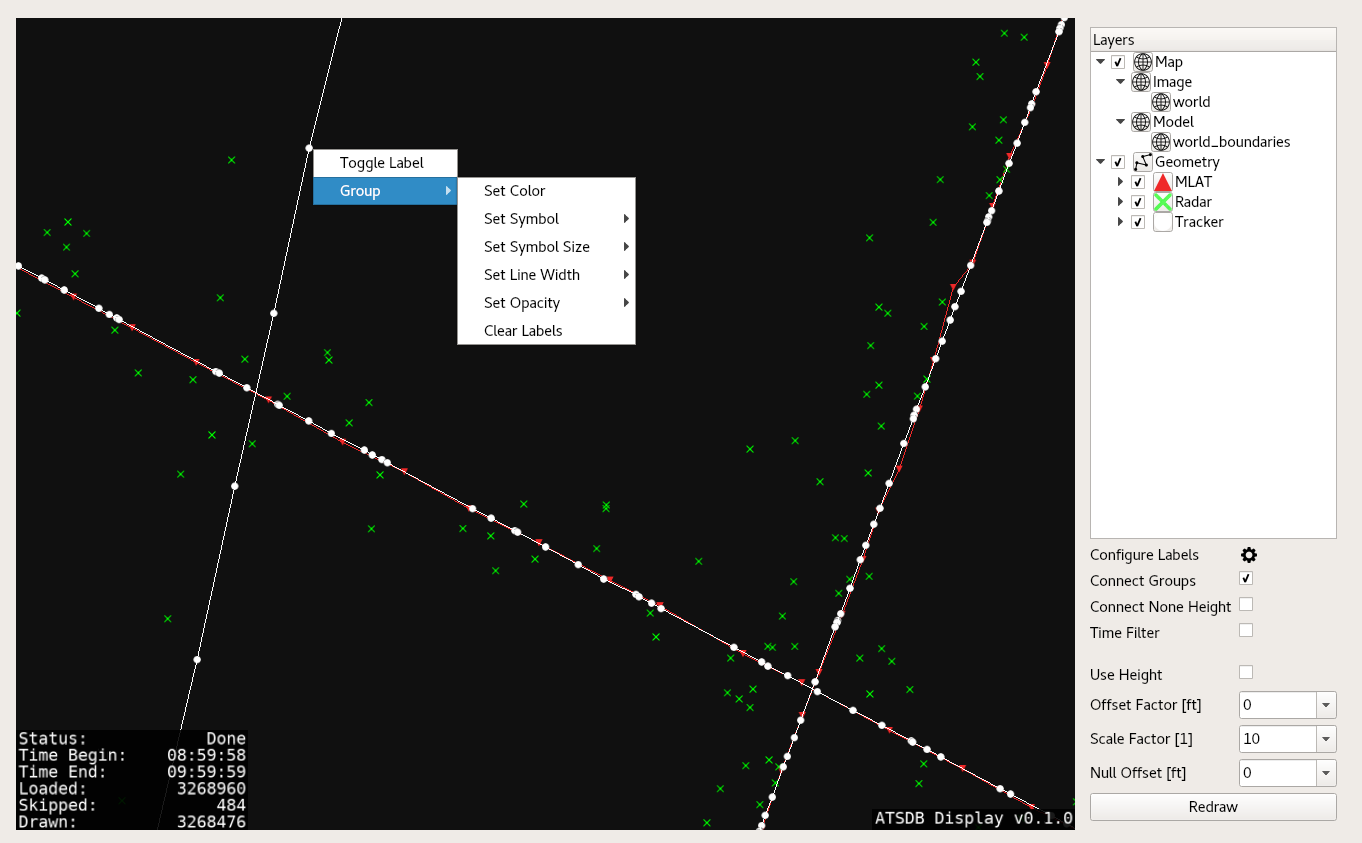
\includegraphics[width=18cm]{../screenshots/osgview_data_operations.png}
  \caption{OSG View data operations}
\end{figure}

The data context menu allows the following operations:

\begin{itemize}
 \item Toogle Label: Toggle label display of a single target report
 \item Group: Same operations as on the item's group layer item
\end{itemize}

\subsubsection{Height Operations}

Per default, a target reports height is not used for display, which is common in current air-traffic displays. However, in certain situation a true 3D display might be of interest to a user, and therefore several options where incorporated:

\begin{itemize}
 \item Use: Use the height based on Mode C $h_c$, transformed to meters
 \item Use Offset: Whether to use an additative height offset
 \item Offset Factor: Height offset value $h_o$
 \item Use Scale: Whether to use an multiplicative factor
 \item Scale Factor: Height scale factor value $h_s$
 \item Connect none: Whether to draw lines to target reports with no height information
\end{itemize}

Generally, if no height information is given (no Mode C code), the height is either $0$ or the height offset (if used). That means that those target reports appear to the on the ground. If connection lines are drawn between the ones in the air and those without, a lot of annoying lines are shown.

The formula to calculate the height is as follows:

$$ h = h_o + h_s \cdot h_c [m]$$ 

Please note that upon changes to the height usage, the complete geometry data is redrawn, which can take several seconds until complete.

\subsubsection{Time Filter}

Once activated, the time filter facilitates that only target reports within a specific time window are shown.


\begin{figure}[H]
    \hspace*{-2cm}
    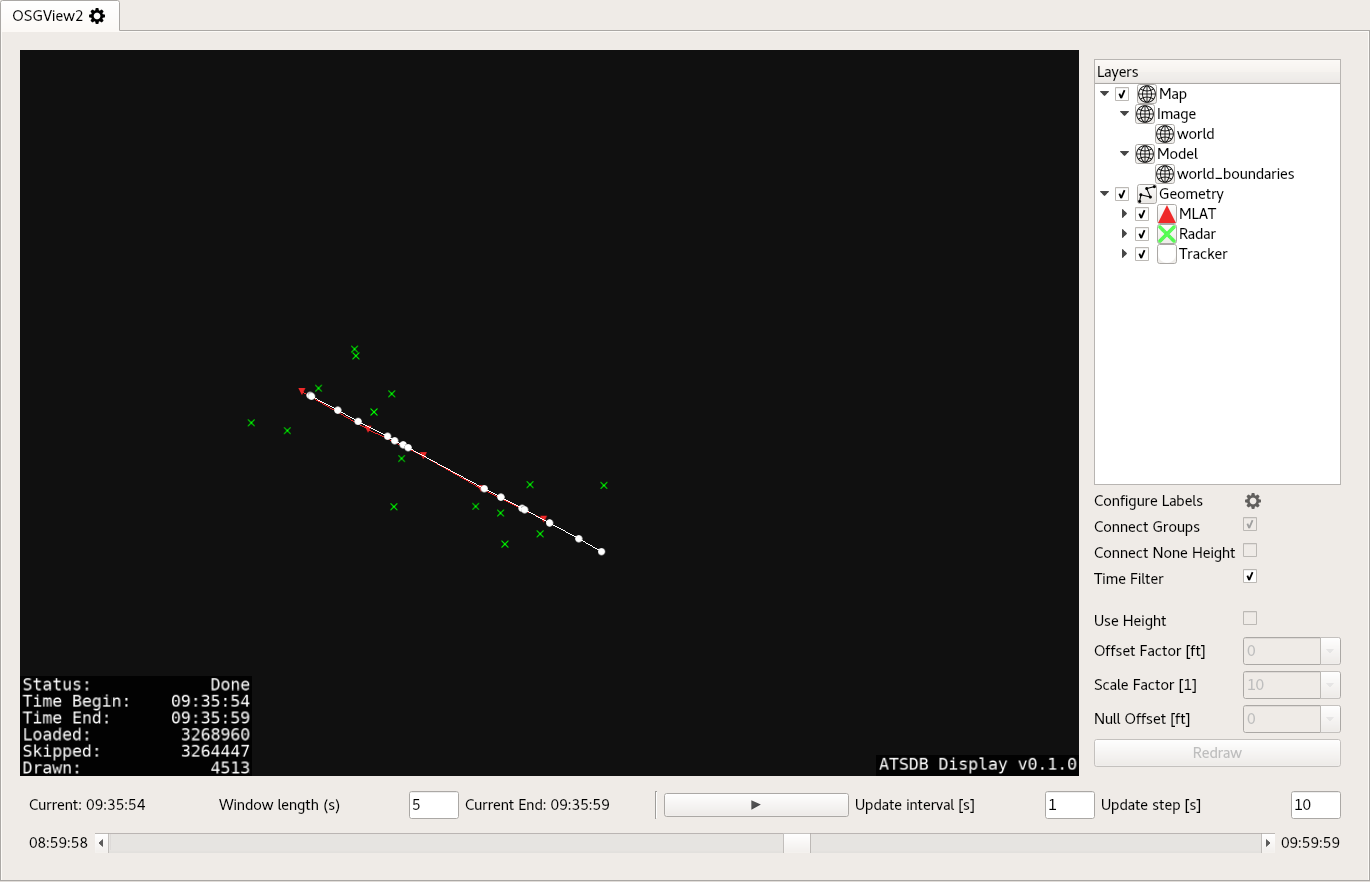
\includegraphics[width=18cm]{../screenshots/osgview_time_filter.png}
  \caption{OSG View time filter}
  \label{fig:osgview_time_filter}
\end{figure}

The following items exist:

\begin{itemize}
 \item Current: The start of the time window
 \item Window length (s): Duration of the display time window
 \item Current End: The end of the time window
 \item Play button: Start/Stop the auto-play mode
 \item Update interval [s]: Auto-play mode update interval
 \item Update step [s]: Auto-play mode update step
 \item Scrollbar: Manual time-scrolling
\end{itemize}

Please note that unfortunatly in the AppImage especially the time filtering is slower than was to be expected. This is currently under investigation.



%\section{Glossary}
%Buffer
%Dynamic data container, e.g. for DBO data items.
%Configurable
%Component which is configurable using an sophisticated XML-based configuration.
%CPU
%Central Processing Unit; main computational unit of any workstation.
%DBO
%DataBaseObject; an object with a set of variables to be stored in and read from the database, e.g. Plots, System Tracks.
%DBO data item
%One item of a specific DBO, e.g. Radar plot message, System Track status update.
%DBO meta variable
%Variable that binds together a number of DBO variables. 
%DBO variable
%Variable that exists in all DBO data items.
%DBStorage
%GPU
%Graphics Processing Unit; main computational unit of a graphics card.
%GUI
%Graphical User Interface
%ListBoxView
%View that displays any DBO data in a table structure.
%Pipeline
%Architectural equivalent of an assemly line, a number of seperate components execute a number of disjoint jobs in %parallel.
%ResultSet
%Collection of DBO data items.
%SASS-C
%Surveillance Analysis Support System for ATC-Centre; A software toolbox developed by EUROCONTROL to provide standardised %methods and tools for assessing the performance of Surveillance
%infrastructures.
%View
%Visualization of aspects of the result set.
%WorkerThread
%Additional thread that executes TransformationJobs.


%%%%%%%%%%%%%%%%%%%%%%%%%%%%%%%%
%%\endinput
%%%%%%%%%%%%%%%%%%%%%%%%%%%%%%%

%%%%%%%%% end mbooka
%%%%%%%%%%%%%%%%%%%%%%%%%%%%%%%%%%%%%%%%%%%%%%%%%%%%%%%%%%%%

% back end
%\backmatter

%\PWnote{2009/07/08}{Changed \cs{toclevel@section} so that Notes 
                    %divisions appear in the bookmarks}
%\makeatletter\renewcommand*{\toclevel@chapter}{-1}\makeatother 
%\makeatletter\renewcommand*{\toclevel@section}{0}\makeatother
%\clearpage
%\printpagenotes
%\clearpage
%\pagestyle{plainmarkruled}
%%\chapterstyle{section}

%\renewcommand*{\begintheglossaryhook}{\small}
%%%\glossaryintoc
%\printglossary


%\clearpage
%\twocolindex
%\pagestyle{index}
%\renewcommand{\chaptermark}[1]{}
%\renewcommand{\preindexhook}{%
%The first page number is usually, but not always, the primary reference to
%the indexed topic.\vskip\onelineskip}
%\indexintoc

%%%\raggedright  does nasty things to index entries
%\printindex

%\onecolindex
%\renewcommand*{\preindexhook}{}
%\renewcommand*{\indexname}{Index of first lines}
%%%\indexintoc
%\printindex[lines]

%\cleardoublepage
%\pagestyle{empty}
%\null\vfil

\end{document}

\endinput

